\documentclass[11pt,a4paper]{article}

% --- 中文与编码 ---
\usepackage[UTF8]{ctex}

% --- 数学 ---
\usepackage{amsmath}
\usepackage{amssymb}
\usepackage{amsthm}
\usepackage{bm}

% --- 插图与表格 ---
\usepackage{graphicx}
\usepackage{booktabs}
\usepackage{multirow}
\usepackage{array}
\usepackage{caption}
\usepackage{subcaption}
\usepackage{float}
\usepackage{placeins}

% --- 页面与版式 ---
\usepackage[top=2.5cm,bottom=2.5cm,left=2.5cm,right=2.5cm]{geometry}
\usepackage{fancyhdr}
\usepackage{hyperref}
\hypersetup{
    colorlinks=true,
    linkcolor=black,
    citecolor=blue,
    urlcolor=blue,
}
\usepackage{cite}

% --- 图表排版 ---
\captionsetup{font=small,labelfont=bf,labelsep=quad,skip=7pt}
\setlength{\textfloatsep}{16pt plus 3pt minus 4pt}
\setlength{\floatsep}{12pt plus 2pt minus 3pt}
\setlength{\intextsep}{12pt plus 2pt minus 3pt}
\renewcommand{\topfraction}{0.88}
\renewcommand{\bottomfraction}{0.70}
\renewcommand{\textfraction}{0.10}
\renewcommand{\floatpagefraction}{0.85}
\newcommand{\widefig}{0.84\textwidth}
\newcommand{\mediumfig}{0.72\textwidth}

% --- 算法 ---
\usepackage{algpseudocode}
\usepackage{algorithm}
\usepackage{listings}

% --- 绘图 ---
\usepackage{tikz}
\usetikzlibrary{arrows,shapes,positioning,calc}

% --- 标题信息 ---
\title{基于稀疏二阶锥规划的火星动力下降轨迹优化}
\author{LShang\\\large 远界征途航天}
\date{\today}

% --- 页眉页脚 ---
\pagestyle{fancy}
\fancyhf{}
\fancyhead[L]{\small 基于稀疏二阶锥规划的火星动力下降轨迹优化}
\fancyhead[R]{\small LShang}
\fancyfoot[C]{\thepage}
\renewcommand{\headrulewidth}{0.4pt}

% --- 定理环境 ---
\newtheorem{theorem}{定理}[section]
\newtheorem{lemma}{引理}[section]
\newtheorem{definition}{定义}[section]
\newtheorem{corollary}{推论}[section]

\begin{document}

\maketitle

\begin{abstract}
本文以火星动力下降段轨迹优化为工程背景，围绕序列锥规划（Sequential Convex Programming, SCP）框架下的二阶锥规划（Second-Order Cone Programming, SOCP）问题展开研究。针对动力下降段中的推力幅值禁带约束、下滑角约束和终端状态约束，采用凸化方法建立标准 SOCP 数值模型。为研究直接求解器接口，本文手工构造稀疏矩阵数据结构，其中等式约束 Jacobian 矩阵包含 733 个非零元，不等式约束 Jacobian 矩阵包含 403 个非零元，运行时不依赖 CVXPY、YALMIP 等通用建模工具。数值对比的证据分为两组：三个 C ECOS 目标可由仓库构建产物直接运行，另有 CVXPY+ECOS、CVXPY+Clarabel 和 CasADi+IPOPT 三条 Python 静态记录。两组在一位小数的燃料目标值上均记录为 400.7~kg；该一致性仅作为实现回归参照，不证明物理可行性或凸化无损性，当前标称解仍存在约 0.728~kg 的干重下界违反。此外，本文在 x86 平台记录了特定构建与计时范围内的求解阶段延迟，为后续部署研究提供限定环境下的基线。
\end{abstract}

% --- 各章引入 ---
\section{引言}

\subsection{研究背景}

火星着陆是深空探测中约束最强的任务阶段之一。苏联 Mars 3 曾实现首次软着陆但很快失联；此后美国与中国完成了可持续运行的火星表面任务\cite{nasaNssdcMars3,govTianwen2021}。动力下降段的起始高度、速度和持续时间随任务设计而变，但共同目标是在有限推进剂、推力和状态约束下满足触地位置与速度要求\cite{braun2007mars}。在此阶段，减速与末端机动主要依赖反推发动机，因此制导算法的鲁棒性、燃料代价和计算时延都必须结合具体任务与硬件验证。

火星科学实验室（MSL）任务在末端下降采用天空起重机方案，以缆绳将"好奇号"火星车放至地面\cite{steltzner2013msl}。Mars 2020 的"毅力号"在 Jezero Crater 着陆；其 EDL 系统包含 Range Trigger、地形相对导航（TRN）和记录下降过程的相机系统\cite{chen2021mars2020}。MEDLI2 传感器套件为进入、下降和着陆环境测量提供了数据。中国于 2021 年 5 月完成天问一号火星着陆任务，祝融号部署在乌托邦平原\cite{govTianwen2021}。这些任务说明，导航、制导、执行器和环境模型必须作为完整 EDL 系统共同验证。

实际动力下降同时受重力、气动、执行器与导航误差影响。本项目采用三自由度平动点质量近似，状态为位置 $r$、速度 $v$ 与对数质量 $\ln m$，并施加终端位置和速度约束。手写基线将六台发动机的单台最小推力 $T_{\min}$ 和留出姿控余量后的单台上界 $T_2=0.8T_{\max}$ 汇总为有效推力包络；它不把发动机关机建成离散决策。该下界造成的非凸性是凸化文献所讨论的问题之一\cite{acikmese2007lossless}。实时重规划的周期、可行性和安全降级策略则取决于目标硬件与闭环场景，不能由本项目的主机基准预先假定。

\subsection{研究现状}

动力下降轨迹优化可采用间接法、直接法和凸优化方法。间接法借助庞特里亚金极大值原理将问题转化为两点边值问题；协态初值、开关结构和路径约束会使数值求解困难。直接法将连续问题转录为有限维非线性规划。伪谱 Legendre 离散可在较少节点上获得高精度近似\cite{el2009legendre}；直接配点则提供分段约束处理的通用途径\cite{benson2003direct}。其规模、收敛性和时延取决于转录方式、约束与求解器设置，是否适合嵌入式使用需要目标问题和硬件上的实测证据。

凸优化方法为部分受限动力下降问题提供可分析的近似或等价表述。Açıkmeşe 和 Ploen 研究了火星动力下降的凸规划表述\cite{acikmese2007lossless}；Blackmore 等人研究了特定非线性最优控制问题的控制约束无损凸化条件\cite{blackmore2012lossless}。Liu、Lu 和 Pan 的 2017 年论文综述了航空航天凸优化应用\cite{liu2017trajectory}。这些结果说明了 SOCP 与序列凸化的理论基础，但本项目的离散、线性化和物理可行性仍须由自身审计而非文献标题推断。

\subsection{现有工作的局限}

工程实现仍需分别处理建模、数值与证据问题。通用建模层便于原型验证，却可能引入建模、规范化和数据转换开销；直接输入求解器矩阵则需要可审查的装配与符号验证。不同求解器、模型版本和运行环境的数值输出只有连同物理残差才具有可比性。单精度与双精度的差异也必须在相同模型、缩放和容差下控制实验，不能由不同配置的单次结果推导硬件选择。

\subsection{本文贡献}

本文在凸优化制导的理论框架下，以火星动力下降轨迹优化为具体场景，给出以下可复核贡献。

（1）\textbf{原始手写稀疏矩阵资产。} \texttt{MarsLanding/MarsLanding.c} 是作者原始、独立、人工维护的 CRS 构造及 CRS--CCS 转换实现。等式约束矩阵含 733 个非零元，不等式约束矩阵含 403 个非零元；自动生成和 Python 路径只承担交叉验证职责，不能覆盖或替代该资产。

（2）\textbf{分组数值对比。} 三个 C ECOS 目标可直接构建运行；另保存三条 Python 对照记录，分别覆盖 ECOS、Clarabel 和 IPOPT。两组均在一位小数目标值上记录为 400.7 kg。该对比用于发现明显实现回归，不声称高精度逐位相等，也不据此证明物理模型正确或凸化无损。

（3）\textbf{物理修正的终端时间研究。} 在保留原始手写基线的同时，建立显式干重与区间内下滑锥约束的参数化 SOCP，并用冻结网格搜索、逐点审计和 ECOS/Clarabel 复算记录可行边界。该研究发现节点可行不等于区间可行，并报告网格敏感性而非宣称连续时间最优。

（4）\textbf{可追溯证据链。} 场景、逐样本记录、聚合结果、claim ledger 和论文图表在仓库中关联；历史 400.7 kg 路径仅作为数值 golden，物理审计、性能和精度结论均明确其测量范围。作为范围受限的主机记录，N150 上 setup 后的 1000 次求解 CPU 时间均值为 7.361 ms。

\subsection{论文组织}

第 2 章定义三自由度模型和物理约定；第 3 章说明凸化、离散化及其适用边界；第 4 章给出原始独立手写 CRS--CCS 资产和 ECOS 接口约定；第 5 章给出分组数值证据、物理修正自由时间研究和主机计时范围；第 6 章界定部署证据与待验证事项；第 7 章总结结论与下一步验证路线。

\section{问题描述与建模}

\subsection{坐标系定义}

本文采用火星固连坐标系（Mars-Centered, Mars-Fixed, MCMF）描述着陆器的运动状态。坐标系原点位于火星质心，$x$轴沿火星径向方向指向上方（远离火星表面），$y$轴和$z$轴位于水平面内，构成右手直角坐标系。在该坐标系下，着陆器的位置向量记为$\bm{r} = [r_x, r_y, r_z]^{\top}$，其中$r_x$表示着陆器距火星参考球面的径向高度，$r_y$和$r_z$表示水平方向的位置分量。速度向量记为$\bm{v} = [v_x, v_y, v_z]^{\top}$，分别对应各轴方向的速度分量。

在动力下降段，着陆器距离火星表面仅数千米，相对于火星半径的尺度而言可近似认为重力加速度为常值。火星表面平均重力加速度为$g = 3.7114\;\mathrm{m/s^2}$，方向沿$x$轴负方向（指向火星表面）。由于动力下降段时间短（$t_f = 81\;\mathrm{s}$）、运动范围小，忽略火星自转效应和科里奥利力的影响，固连坐标系可视为惯性系。

\subsection{物理参数}

本文所研究的火星动力下降段着陆器物理参数如表\ref{tab:params}所示。

\begin{table}[H]
    \centering
    \caption{火星动力下降段物理参数}
    \label{tab:params}
    \begin{tabular}{cll}
        \toprule
        符号 & 物理意义 & 数值 \\
        \midrule
        $g$          & 火星表面重力加速度                      & $3.7114\;\mathrm{m/s^2}$ \\
        $I_{\mathrm{sp}}$ & 发动机比冲                      & $225\;\mathrm{s}$ \\
        $m_0$        & 初始总质量                              & $1905\;\mathrm{kg}$ \\
        $m_{\mathrm{dry}}$ & 干重（结构质量）                  & $1505\;\mathrm{kg}$ \\
        $T_{\max}$   & 单台发动机最大推力                        & $3100\;\mathrm{N}$ \\
        $T_2$        & 姿控可用最大推力 ($0.8\,T_{\max}$)       & $2480\;\mathrm{N}$ \\
        $n_T$        & 发动机台数                              & $6$ \\
        $\phi$       & 发动机安装倾角                            & $27^\circ$ \\
        $\theta$     & 最大下滑角                              & $86^\circ$ \\
        $N$          & 离散控制段数                            & $30$ \\
        $t_f$        & 给定着陆时间                            & $81\;\mathrm{s}$ \\
        $\bm{r}_0$   & 初始位置 $[r_{x0}, r_{y0}, r_{z0}]^{\top}$ & $[1500, 0, 2000]^{\top}\;\mathrm{m}$ \\
        $\bm{v}_0$   & 初始速度 $[v_{x0}, v_{y0}, v_{z0}]^{\top}$ & $[-75, 0, 100]^{\top}\;\mathrm{m/s}$ \\
        \bottomrule
    \end{tabular}
\end{table}

其中，$g$为火星表面重力加速度，取值$3.7114\;\mathrm{m/s^2}$约为地球重力加速度的$0.378$倍。$I_{\mathrm{sp}}$为发动机比冲，表征推进系统的燃料效率，取值$225\;\mathrm{s}$对应于典型液体燃料发动机的性能水平。$m_0$为初始总质量，$m_{\mathrm{dry}}$为干重（结构质量），二者之差$\Delta m = 400\;\mathrm{kg}$即为可用燃料质量。$T_{\max}$为单台发动机最大推力，而$T_2 = 0.8\,T_{\max}$为扣除$20\%$姿控余量后可用于动力下降的推力上界——这$20\%$的余量确保姿态控制系统在动力下降过程中有足够的力矩裕度。$n_T = 6$为发动机台数，均布于着陆器底部。$\phi = 27^\circ$为发动机喷管轴线与着陆器中心轴线之间的安装倾角，该倾斜布局使得发动机在提供轴向推力的同时具备水平方向推力分量，从而实现对水平速度的直接控制。$\theta = 86^\circ$为最大允许下滑角，保证着陆轨迹近乎垂直，防止着陆器因水平速度过大而倾覆。$N = 30$为用于数值求解的离散控制段数，$t_f = 81\;\mathrm{s}$为给定的着陆时间。

初始位置$\bm{r}_0 = [1500, 0, 2000]^{\top}\;\mathrm{m}$意味着着陆器在动力下降开始时位于目标着陆点正上方$1500\;\mathrm{m}$，同时在$z$方向有$2000\;\mathrm{m}$的水平偏移。初始速度$\bm{v}_0 = [-75, 0, 100]^{\top}\;\mathrm{m/s}$表明着陆器已有$75\;\mathrm{m/s}$的竖直向下速度分量和$100\;\mathrm{m/s}$的$z$方向水平速度。

\subsection{三自由度动力学方程}

在火星固连坐标系下，着陆器被视为变质量质点，其三自由度动力学方程由牛顿第二定律和变质量系统的质量守恒律推导得到。连续时间动力学方程组为
\begin{align}
    \dot{\bm{r}} &= \bm{v}, \label{eq:dr} \\
    \dot{\bm{v}} &= \bm{g} + \frac{\bm{T}_{\mathrm{total}}}{m}, \label{eq:dv} \\
    \dot{m}      &= -\alpha \left\|\bm{T}_{\mathrm{total}}\right\|, \label{eq:dm}
\end{align}
其中$\bm{T}_{\mathrm{total}} = [T_x, T_y, T_z]^{\top}$为$n_T$台发动机产生的总推力向量，$\bm{g} = [-g, 0, 0]^{\top}$为重力加速度向量，$m$为着陆器当前时刻的瞬时质量。

式\eqref{eq:dr}是位置与速度之间的运动学关系，式\eqref{eq:dv}是牛顿第二定律的矢量形式——着陆器加速度由重力项和控制加速度项（推力除以质量）两部分构成。式\eqref{eq:dm}为质量消耗方程，描述了推进剂消耗速率与推力幅值之间的正比关系。

系数$\alpha$为单位推力幅值对应的质量消耗率。根据火箭发动机比冲定义，推力幅值与推进剂质量流率的关系为
\begin{align}
    \|\bm{T}_{\mathrm{total}}\| = n_T\,I_{\mathrm{sp}}\,g_0\,(-\dot{m}/n_T)\cos\phi
                               = I_{\mathrm{sp}}\,g_0\,(-\dot{m})\cos\phi,
\end{align}
其中$g_0 = 9.80665\;\mathrm{m/s^2}$为地球标准重力加速度（用于比冲定义），$\cos\phi$因子来源于发动机推力沿轴向的分量。整理得
\begin{align}
    \dot{m} = -\frac{\|\bm{T}_{\mathrm{total}}\|}{I_{\mathrm{sp}}\,g_0\cos\phi}
            \triangleq -\alpha\,\|\bm{T}_{\mathrm{total}}\|,
    \qquad
    \alpha = \frac{1}{I_{\mathrm{sp}}\,g_0\cos\phi}. \label{eq:alpha}
\end{align}
该定义与代码实现~\cite{blackmore2010minimum}\cite{acikmese2007lossless}一致（见\texttt{mars\_params.py}: \texttt{alpha = 1.0/(I\_sp * g\_earth * cos(phi))}）。

将式\eqref{eq:dv}按各轴分量展开，得到三个标量微分方程：
\begin{align}
    \dot{v}_x &= -g + \frac{T_x}{m}, \label{eq:dvx} \\
    \dot{v}_y &= \frac{T_y}{m}, \label{eq:dvy} \\
    \dot{v}_z &= \frac{T_z}{m}. \label{eq:dvz}
\end{align}

式\eqref{eq:dvx}中重力加速度$g$带负号，代表重力指向火星表面（即$x$轴负方向）。着陆器要想减速并最终悬浮于目标点，必须依靠推力分量$T_x$提供足够大的向上的加速度，以抵消重力并产生减速效果。当$T_x > mg$时，着陆器在$x$方向获得向上的净加速度，$|v_x|$逐渐减小至零。$y$和$z$方向无重力项，水平面的运动加速度完全由推力分量决定。

从式\eqref{eq:dv}对时间积分，可以得到速度增量的近似表达式：
\begin{align}
    \bm{v}(t) - \bm{v}_0 = \bm{g}\,t + \int_0^{t} \frac{\bm{T}_{\mathrm{total}}(\tau)}{m(\tau)}\,\mathrm{d}\tau.
\end{align}

可见着陆器在动力下降过程中需要克服重力作用，同时通过调节推力矢量补偿初始速度偏差，最终达到终端零速度的条件。

\subsection{控制量与推力矢量关系}

\subsubsection{发动机配置}

着陆器底部均布安装$n_T = 6$台液体火箭发动机，每台发动机的推力大小可独立调节，且具备深度节流能力。各发动机的安装轴线与着陆器中心轴线（$x$轴）之间具有相同的安装倾角$\phi = 27^\circ$，即每台发动机的推力方向均偏离$x$轴一个固定角度$\phi$，且在水平面内均匀分布，相邻两台发动机之间夹角为$60^\circ$。

设第$i$台发动机的推力大小为$T_i\;(i = 1, 2, \ldots, n_T)$，其推力向量在火星固连坐标系中的分解为
\begin{align}
    \bm{T}_i = T_i
    \begin{bmatrix}
        \cos\phi \\
        \sin\phi\,\cos\psi_i \\
        \sin\phi\,\sin\psi_i
    \end{bmatrix},
\end{align}
其中$\psi_i = (i-1)\times 60^\circ$为第$i$台发动机轴线在水平面内投影的方位角。各台发动机的方位角具体为
\begin{align}
    \psi_i \in \{0^\circ,\; 60^\circ,\; 120^\circ,\; 180^\circ,\; 240^\circ,\; 300^\circ\}.
\end{align}

$n_T$台发动机的总推力向量为各台推力向量之和：
\begin{align}
    \bm{T}_{\mathrm{total}} = \sum_{i=1}^{n_T} \bm{T}_i =
    \begin{bmatrix}
        \displaystyle\sum_{i=1}^{n_T} T_i\cos\phi \\[6pt]
        \displaystyle\sum_{i=1}^{n_T} T_i\sin\phi\,\cos\psi_i \\[6pt]
        \displaystyle\sum_{i=1}^{n_T} T_i\sin\phi\,\sin\psi_i
    \end{bmatrix}. \label{eq:Ttotal}
\end{align}

\subsubsection{加速度控制量}

为简化控制问题的表述，引入加速度控制量$\bm{u} = [u_x, u_y, u_z]^{\top}$，其定义为总推力向量除以当前质量：
\begin{align}
    \bm{u} = \frac{\bm{T}_{\mathrm{total}}}{m}. \label{eq:u_def}
\end{align}

将式\eqref{eq:Ttotal}代入式\eqref{eq:u_def}，可得加速度控制量的各轴分量表达式为
\begin{align}
    u_x &= \frac{\cos\phi}{m}\sum_{i=1}^{n_T} T_i, \\
    u_y &= \frac{\sin\phi}{m}\sum_{i=1}^{n_T} T_i\cos\psi_i, \\
    u_z &= \frac{\sin\phi}{m}\sum_{i=1}^{n_T} T_i\sin\psi_i.
\end{align}

当6台发动机推力不等时，总推力矢量的方向可在一定范围内连续变化。令$\bm{e}_i = [\cos\phi,\;\sin\phi\cos\psi_i,\;\sin\phi\sin\psi_i]^{\top}$，则总推力矢量可控空间为
\begin{align}
    \bm{T}_{\mathrm{total}} \in \left\{ \sum_{i=1}^{n_T} T_i\,\bm{e}_i \;:\; T_i \in [T_{\min},\, T_{\max}] \right\}.
\end{align}

由于$n_T = 6$且$\bm{e}_i$在三维空间中张成了多面锥，总推力矢量的可达集是一个以$x$轴为对称轴的多边形锥体。对于本文所考虑的燃料最优轨迹规划问题，进一步假设各发动机同步调节，即每台发动机的推力大小相等：
\begin{align}
    T_1 = T_2 = \cdots = T_{n_T} = T.
\end{align}

此时总推力矢量方向由几何配置唯一确定，各轴分量简化为
\begin{align}
    T_x &= n_T\,T\cos\phi, \\
    T_y &= n_T\,T\sin\phi\cdot\frac{1}{6}\sum_{i=1}^{6}\cos\psi_i = 0, \\
    T_z &= n_T\,T\sin\phi\cdot\frac{1}{6}\sum_{i=1}^{6}\sin\psi_i = 0.
\end{align}

由于余弦和正弦在完整圆周上的对称性，$\sum\cos\psi_i = \sum\sin\psi_i = 0$，均布推力时水平分量互相抵消，总推力方向仅沿$x$轴方向。但在非同步调节的一般情况下，通过调制各台发动机的推力差异，可以在水平面内产生净推力分量，从而实现水平方向的速度控制。本文采用等效总推力向量$\bm{T} = [T_x, T_y, T_z]^{\top}$作为实际设计变量，直接表示总推力在各轴上的分量，令加速度控制量$\bm{u}$为
\begin{align}
    u_x = \frac{T_x}{m},\qquad
    u_y = \frac{T_y}{m},\qquad
    u_z = \frac{T_z}{m}. \label{eq:u_comp}
\end{align}

将式\eqref{eq:u_def}与\eqref{eq:alpha}代入质量消耗方程\eqref{eq:dm}，得到以加速度控制量表示的质量变化率：
\begin{align}
    \dot{m} = -\alpha\,m\|\bm{u}\|. \label{eq:dm_u}
\end{align}

至此，以$\bm{r}$、$\bm{v}$、$m$为状态变量，以$\bm{u}$为控制变量的连续时间动力学方程组综合如下：
\begin{align}
    \dot{\bm{r}} &= \bm{v}, \label{eq:sys1} \\
    \dot{\bm{v}} &= \bm{g} + \bm{u}, \label{eq:sys2} \\
    \dot{m}      &= -\alpha\,m\|\bm{u}\|. \label{eq:sys3}
\end{align}

式\eqref{eq:sys3}是微分方程中唯一的非线性项，其右端包含了状态$m$与控制量$\bm{u}$的耦合乘积$\|\bm{u}\|$，是该最优控制问题非线性的主要来源，也是后续松弛和凸化处理的关键对象。

\subsection{约束条件}

\subsubsection{推力幅值约束}

每台液体火箭发动机的推力大小受到物理限制，只能在最小推力$T_{\min}$和最大推力$T_{\max}$之间连续调节：
\begin{align}
    T_{\min} \leq T_i \leq T_{\max}, \quad i = 1, 2, \ldots, n_T. \label{eq:Ti_bound}
\end{align}

需要说明的是，对于液体火箭发动机，$T_{\min}$通常不为零，而是受到燃烧室稳定工作条件的限制（典型值为$30\%$额定推力）。但在动力下降段的数学规划中，通常不对$T_{\min}$施加严格的下界约束，而是依靠最优解的自然特性保证发动机工作在合理区间。

考虑工程实际，需要预留$20\%$的推力用于姿态控制系统，因此实际可用于动力下降的可用最大推力为
\begin{align}
    T_2 = 0.8\,T_{\max} = 2480\;\mathrm{N}.
\end{align}

由$n_T$台发动机的总推力幅值$\|\bm{T}_{\mathrm{total}}\|$满足的约束为
\begin{align}
    0 \leq \|\bm{T}_{\mathrm{total}}\| \leq n_T\,T_2. \label{eq:T_norm_bound}
\end{align}

将式\eqref{eq:u_def}代入上式，得到关于加速度控制量$\bm{u}$的约束：
\begin{align}
    0 \leq \|\bm{u}\| \leq \frac{n_T\,T_2}{m}. \label{eq:u_bound}
\end{align}

注意到该约束的上界与状态变量$m$有关，属于状态相关的控制约束（state-dependent control constraint）。随着推进剂的消耗，$m$逐渐减小，约束上界$\frac{n_T T_2}{m}$逐渐增大，意味着后期可用加速度更大。

\subsubsection{下滑角约束}

为保证着陆器以近乎垂直的姿态安全着陆，避免因水平速度过大导致着陆时倾覆，需对飞行轨迹的下滑角施加约束。下滑角定义为速度向量与水平面之间的夹角$\gamma$，满足
\begin{align}
    \tan\gamma = \frac{-v_x}{\sqrt{v_y^2 + v_z^2}}.
\end{align}

该约束等价于要求速度方向始终保持在以$x$轴为对称轴的一个倒锥体内。在仅给定初始和终端位置的情况下，更常用的是路径约束形式——位置空间中的锥形约束，以确保着陆器始终保持在安全走廊内：
\begin{align}
    \sqrt{r_y^2 + r_z^2} \leq r_x \tan\theta, \label{eq:glideslope}
\end{align}
其中$\theta = 86^\circ$为最大允许下滑角，$\tan 86^\circ \approx 14.30$。该约束的几何意义如图\ref{fig:glideslope}所示，它定义了以$x$轴线为中心轴、半顶角为$86^\circ$的倒锥形安全走廊，着陆器的三维位置$[r_x, r_y, r_z]$必须在锥体内部。

\begin{figure}[H]
    \centering
    \begin{tikzpicture}[scale=0.6]
        \draw[->] (0,0) -- (5,0) node[right]{$r_y$};
        \draw[->] (0,0) -- (0,5) node[above]{$r_x$};
        \draw[->] (0,0) -- (-2,-1) node[below]{$r_z$};
        \draw[dashed] (0,0) -- (4, {4*tan(86)});
        \draw[dashed] (0,0) -- (4, -{4*tan(86)});
        \draw[->] (1,0) arc (0:86:1) node[right]{$\theta$};
        \fill (3,2) circle (0.08);
        \node at (3.5,2.3){着陆器};
    \end{tikzpicture}
    \caption{下滑角约束的几何示意图}
    \label{fig:glideslope}
\end{figure}

将$\theta = 86^\circ$代入式\eqref{eq:glideslope}，得到具体的约束不等式为
\begin{align}
    \sqrt{r_y^2 + r_z^2} \leq 14.30\,r_x. \label{eq:glideslope_num}
\end{align}

对于初始位置$r_{x0} = 1500\;\mathrm{m}$，水平方向最大允许偏移量为$14.30 \times 1500 \approx 21450\;\mathrm{m}$——远大于实际的初始水平偏移$2000\;\mathrm{m}$。因此，该约束在动力下降的前期和中段并不活跃，它的主要作用是约束终端段的飞行姿态：随着$r_x$趋近于零，允许的水平偏移范围也迅速缩小，保证着陆器最终以近似垂直的状态抵达着陆点。

在优化问题的数值求解中，下滑角约束\eqref{eq:glideslope}是一个典型的二阶锥约束，可写为以下标准形式：
\begin{align}
    \|[r_y,\; r_z]^{\top}\| \leq r_x\tan\theta.
\end{align}

\subsubsection{质量约束}

着陆器在动力下降过程中的质量受物理极限的约束，其取值范围为
\begin{align}
    m_{\mathrm{dry}} \leq m(t) \leq m_0, \quad \forall t \in [0, t_f]. \label{eq:mass_bound}
\end{align}

其中$m_{\mathrm{dry}} = 1505\;\mathrm{kg}$为着陆器结构干重，包含着陆器本体结构、有效载荷和未消耗的残余推进剂的质量。$m_0 = 1905\;\mathrm{kg}$为动力下降开始时的初始总质量，由进入段末端的状态确定。质量差$\Delta m = m_0 - m_{\mathrm{dry}} = 400\;\mathrm{kg}$即为可用于动力下降的燃料总储备。在燃料最优轨迹规划中，终端质量$m(t_f)$越接近$m_{\mathrm{dry}}$，意味着燃料消耗越接近于可用燃料储备。

\subsubsection{边界条件}

动力下降段的初始状态由导航系统在进入段末端给出的测量值确定，是固定的已知量：
\begin{align}
    \bm{r}(0) &= \bm{r}_0 = [1500,\;0,\;2000]^{\top}\;\mathrm{m}, \\
    \bm{v}(0) &= \bm{v}_0 = [-75,\;0,\;100]^{\top}\;\mathrm{m/s}, \\
    m(0)     &= m_0 = 1905\;\mathrm{kg}. \label{eq:init_cond}
\end{align}

终端状态要求着陆器在给定着陆时刻$t_f = 81\;\mathrm{s}$以零速度精确到达目标着陆点（火星固连坐标系原点）：
\begin{align}
    \bm{r}(t_f) &= \bm{0}, \\
    \bm{v}(t_f) &= \bm{0}. \label{eq:term_cond}
\end{align}

终端质量不作约束，由动力学方程自然演化确定，但自动满足$m(t_f) \geq m_{\mathrm{dry}}$。

\subsection{燃料最优目标函数}

在火星动力下降任务中，推进剂是最宝贵的资源。有效载荷质量与燃料消耗直接相关，因此燃料最优化是轨迹规划的核心目标。

燃料消耗总量等于初始质量减去终端质量：
\begin{align}
    J = m_0 - m(t_f).
\end{align}

利用式\eqref{eq:dm}将终端质量表示为对质量变化率的积分：
\begin{align}
    m(t_f) = m_0 + \int_0^{t_f} \dot{m}(t)\,\mathrm{d}t
           = m_0 - \int_0^{t_f} \alpha \left\|\bm{T}_{\mathrm{total}}(t)\right\|\,\mathrm{d}t.
\end{align}

代入$J$的表达式，得到
\begin{align}
    J = \int_0^{t_f} \alpha \left\|\bm{T}_{\mathrm{total}}(t)\right\|\,\mathrm{d}t. \label{eq:cost_full}
\end{align}

由于$\alpha$为正常数，燃料最优等价于最小化总推力对时间的积分，即推力总冲（total impulse）：
\begin{align}
    \min\; J = \int_0^{t_f} \left\|\bm{T}_{\mathrm{total}}(t)\right\|\,\mathrm{d}t. \label{eq:cost_fuel}
\end{align}

此目标函数的物理意义直观明确：减小任意时刻的推力幅值或缩短推力作用时间均可降低燃料消耗。但由于终端时间$t_f$固定，质心在缩短推力时间，这意味着需要增大推力幅值以提供足够的减速度，从而产生了推力大小与作用时间之间的折中关系。

将式\eqref{eq:u_def}代入式\eqref{eq:cost_fuel}，得到以加速度控制量$\bm{u}$表示的目标函数：
\begin{align}
    \min\; J = \int_0^{t_f} m(t)\left\|\bm{u}(t)\right\|\,\mathrm{d}t. \label{eq:cost_u}
\end{align}

该表达式中含有状态量$m(t)$与控制量$\bm{u}(t)$的乘积项，进一步体现了目标函数的非线性特性。

\subsection{Bolza型最优控制问题}

综合上述动力学方程、约束条件和目标函数，火星动力下降燃料最优轨迹规划问题最终可表述为以下连续时间最优控制问题的标准Bolza形式。

\textbf{状态变量:}
\begin{align}
    \bm{x}(t) = [\bm{r}(t)^{\top},\; \bm{v}(t)^{\top},\; m(t)]^{\top} \in \mathbb{R}^7.
\end{align}

\textbf{控制变量:}
\begin{align}
    \bm{u}(t) = [u_x(t),\; u_y(t),\; u_z(t)]^{\top} \in \mathbb{R}^3.
\end{align}

\textbf{动力学方程:}
\begin{align}
    \dot{\bm{x}} = \bm{f}(\bm{x}, \bm{u}) =
    \begin{bmatrix}
        \bm{v} \\
        \bm{g} + \bm{u} \\
        -\alpha\,m\|\bm{u}\|
    \end{bmatrix}. \label{eq:bolza_dyn}
\end{align}

\textbf{路径约束:}
\begin{align}
    \left\|\bm{u}(t)\right\| &\leq \frac{n_T T_2}{m(t)}, \label{eq:bolza_path1} \\
    \sqrt{r_y^2 + r_z^2}    &\leq r_x \tan\theta, \label{eq:bolza_path2} \\
    m_{\mathrm{dry}}        &\leq m(t) \leq m_0. \label{eq:bolza_path3}
\end{align}

\textbf{边界条件:}
\begin{align}
    \bm{x}(0) &= [\bm{r}_0^{\top},\; \bm{v}_0^{\top},\; m_0]^{\top}, \label{eq:bolza_bc1} \\
    \bm{r}(t_f) &= \bm{0},\quad \bm{v}(t_f) = \bm{0}. \label{eq:bolza_bc2}
\end{align}

\textbf{目标函数（Lagrange型）:}
\begin{align}
    \min\; J = \int_0^{t_f} \mathcal{L}(\bm{x}, \bm{u})\,\mathrm{d}t, \label{eq:bolza_cost}
\end{align}
其中Lagrange函数为
\begin{align}
    \mathcal{L}(\bm{x}, \bm{u}) = m(t)\left\|\bm{u}(t)\right\|. \label{eq:lagrangian}
\end{align}

由于式\eqref{eq:bolza_cost}中仅含有运行代价积分项而终端代价为零，该问题在严格意义上属于Lagrange型最优控制问题，但其结构可以视为Bolza型（含积分代价+终端代价）的一个特例。

式\eqref{eq:bolza_dyn}--\eqref{eq:bolza_cost}构成完整的连续时间最优控制问题。利用庞特里亚金极小值原理（Pontryagin's Minimum Principle）分析该问题的结构，可揭示其最优解的理论特征。定义Hamiltonian函数：
\begin{align}
    \mathcal{H}(\bm{x}, \bm{u}, \bm{\lambda}) = m\|\bm{u}\| + \bm{\lambda}_r^{\top}\bm{v} + \bm{\lambda}_v^{\top}(\bm{g} + \bm{u}) - \lambda_m\,\alpha\,m\|\bm{u}\|,
\end{align}
其中$\bm{\lambda} = [\bm{\lambda}_r^{\top},\, \bm{\lambda}_v^{\top},\, \lambda_m]^{\top}$为协态向量（costate）。根据极小值原理，最优控制量$\bm{u}^*$在每一时刻应最小化Hamiltonian函数：
\begin{align}
    \bm{u}^* = \arg\min_{\|\bm{u}\| \leq n_T T_2/m} \left[ m\|\bm{u}\| + \bm{\lambda}_v^{\top}\bm{u} - \lambda_m\,\alpha\,m\|\bm{u}\| \right].
\end{align}

整理关于$\|\bm{u}\|$的系数可知，最优控制的开关结构由协态的演化轨迹决定。这一分析揭示了最优推力幅值和方向的控制律结构，为后续章节直接法的离散化方案和松弛策略提供了理论参照。

该问题具有以下数学特征：
\begin{enumerate}
    \item \textbf{非线性动力学:} 式\eqref{eq:bolza_dyn}中质量变化率方程包含状态与控制量的耦合项$m\|\bm{u}\|$，使系统呈现本质非线性；
    \item \textbf{非凸控制约束:} 式\eqref{eq:bolza_path1}中控制约束的上界依赖于状态$m(t)$，属于状态相关的控制约束（state-dependent constraint），导致可行域非凸；
    \item \textbf{二阶锥约束:} 下滑角约束\eqref{eq:bolza_path2}是典型的二阶锥约束，形式为$\|[\cdot]\| \leq \text{linear expression}$；
    \item \textbf{自由终端质量:} 终端质量由动力学自然确定，仅受不等式下界约束$m(t_f) \geq m_{\mathrm{dry}}$；
    \item \textbf{多约束耦合:} 路径约束与动力学方程之间存在复杂的相互耦合关系，例如推力上界约束的松紧程度取决于当前质量，而质量又由推力积分决定。
\end{enumerate}

由于上述非线性和多约束耦合特性，该问题的解析求解极为困难。传统间接法虽然能通过求解两点边值问题得到最优解，但面对多约束和状态相关约束时，初值猜测极为敏感，收敛十分困难。直接法将连续时间控制问题进行离散化，将其转化为有限维参数优化问题，具有更强的鲁棒性，是工程实践中的主流方法。

本文后续章节将基于凸优化理论，通过对上述最优控制问题进行凸化松弛和离散化处理，将其转化为可高效求解的二阶锥规划（Second-Order Cone Programming, SOCP）问题。转化路径包含三个关键步骤。

\textbf{步骤一：变量替换。}引入新状态变量$z(t) = \ln m(t)$，对式\eqref{eq:sys3}进行对数变换：
\begin{align}
    \dot{z} = \frac{\dot{m}}{m} = -\alpha\|\bm{u}\|. \label{eq:log_mass}
\end{align}
变换后，质量动力学方程变为关于$z$的线性微分方程，消除了原方程中状态与控制量的乘积耦合。同时，质量约束\eqref{eq:bolza_path3}转化为$z$的线性约束：
\begin{align}
    \ln m_{\mathrm{dry}} \leq z(t) \leq \ln m_0.
\end{align}

\textbf{步骤二：约束松弛。}推力上界约束\eqref{eq:bolza_path1}在变量替换后变为
\begin{align}
    \|\bm{u}(t)\| \leq n_T T_2\,e^{-z(t)},
\end{align}
该约束的右端项$e^{-z(t)}$关于$z$是凸函数，但以$z$为自变量的形式使得约束集仍然非凸。通过引入松弛变量$\sigma(t) \geq \|\bm{u}(t)\|$并利用$e^{-z}$的凸性进行序列线性化或直接写作SOC约束，可将该非凸约束转化为凸约束近似。同时需要证明松弛的最优性，即最优解处$\sigma(t) = \|\bm{u}(t)\|$严格成立。

\textbf{步骤三：直接转录。}将时间区间$[0, t_f]$等分为$N$个子区间，在每个子区间上采用零阶保持（Zero-Order Hold, ZOH）离散化策略，即控制量在每一段内保持为常值。利用梯形法或欧拉法对微分方程进行数值积分，得到一组等式约束（即动力学配点约束）。最终获得一个标准SOCP问题，可直接利用内点法求解器（如ECOS、Clarabel等）高效求解。

上述三个步骤构成完整的问题转化链条。在第\ref{chap:convexification}章中，将详细阐述每一步的数学推导细节，包括松弛紧性的严格证明和离散化误差分析。

\subsection{无量纲化处理}

为改善数值求解的收敛性和计算精度，对上述最优控制问题中的状态变量和控制变量进行无量纲化处理。引入无量纲基准量：位置基准$r_{\mathrm{ref}} = r_{x0} = 1500\;\mathrm{m}$，质量基准$m_{\mathrm{ref}} = m_0 = 1905\;\mathrm{kg}$，时间基准$t_{\mathrm{ref}} = 1\;\mathrm{s}$。无量纲变量定义为：
\begin{align}
    \bar{\bm{r}} &= \frac{\bm{r}}{r_{\mathrm{ref}}}, &
    \bar{\bm{v}} &= \frac{\bm{v}\,t_{\mathrm{ref}}}{r_{\mathrm{ref}}}, &
    \bar{m}      &= \frac{m}{m_{\mathrm{ref}}}, &
    \bar{t}      &= \frac{t}{t_{\mathrm{ref}}}, \\
    \bar{\bm{u}} &= \frac{\bm{u}\,t_{\mathrm{ref}}^2}{r_{\mathrm{ref}}}, &
    \bar{g}      &= \frac{g\,t_{\mathrm{ref}}^2}{r_{\mathrm{ref}}}, &
    \bar{\alpha} &= \frac{\alpha\,m_{\mathrm{ref}}\,r_{\mathrm{ref}}}{t_{\mathrm{ref}}^2}.
\end{align}

代入式\eqref{eq:sys1}--\eqref{eq:sys3}，得到无量纲动力学方程：
\begin{align}
    \frac{\mathrm{d}\bar{\bm{r}}}{\mathrm{d}\bar{t}} &= \bar{\bm{v}}, \\
    \frac{\mathrm{d}\bar{\bm{v}}}{\mathrm{d}\bar{t}} &= \bar{\bm{g}} + \bar{\bm{u}}, \\
    \frac{\mathrm{d}\bar{m}}{\mathrm{d}\bar{t}} &= -\bar{\alpha}\,\bar{m}\|\bar{\bm{u}}\|.
\end{align}

无量纲化处理后，位置变量量级约为$O(1)$，速度变量量级约为$O(10^{-1})$，质量变量量级为$O(1)$，控制变量量级约为$O(10^{-3})$。各变量数值范围得到大幅压缩，与求解器内部默认的数值容差（通常在$10^{-8}$到$10^{-6}$之间）相匹配，有效提高了数值优化的收敛性和计算精度。此外，无量纲化还消除了物理单位不统一可能引入的数值误差。本文后续章节的数值求解均采用无量纲化后的变量。

\section{无损凸化与离散化}\label{chap:convexification}\label{sec:convexification}

本章说明将给定网格上的燃料最优着陆候选问题转化为二阶锥规划（SOCP）的过程：变量变换、锥松弛、质量包络线性化和直接转录。Lossless Convexification 文献理论用于界定松弛紧性的充分条件；本项目具体离散模型的物理可行性仍由第 5 章的独立审计判定。

\subsection{凸化动机与问题描述}

\subsubsection{原始最优控制问题}

考虑三维空间中的火箭动力着陆问题。定义状态变量为位置矢量~$\bm r(t)\in\mathbb{R}^3$、速度矢量~$\bm v(t)\in\mathbb{R}^3$和质量~$m(t)\in\mathbb{R}_+$，控制变量为推力矢量~$\bm T(t)\in\mathbb{R}^3$。在常值重力场中，系统的连续时间动力学方程为：
\begin{align}
\dot{\bm r} &= \bm v,\label{eq:dyn_r}\\
\dot{\bm v} &= \bm g + \frac{\bm T}{m},\label{eq:dyn_v}\\
\dot m &= -\alpha\|\bm T\|,\label{eq:dyn_m}
\end{align}
其中~$\bm g=[-g,0,0]^{\mathsf T}$为重力加速度矢量（$g=3.7114~\text{m/s}^2$），$\alpha=1/(I_{\text{sp}}g_0\cos\phi)$为推力比冲相关的常数（$I_{\text{sp}}$为比冲，$g_0$为海平面重力加速度）。初始条件与终端条件分别为：
\begin{align}
\bm r(0) &=\bm r_0,\quad \bm v(0) =\bm v_0,\quad m(0)=m_0,\\
\bm r(t_f) &=\bm r_f,\quad \bm v(t_f)=\bm v_f,
\end{align}
其中~$t_f$为总飞行时间，$\bm r_f$为目标着陆点位置，$\bm v_f= \bm 0$为着陆速度（软着陆条件）。推力幅值受到物理限制：
\begin{align}
T_{\min} \le \|\bm T(t)\| \le T_{\max},\quad \forall t\in[0,t_f],
\end{align}
其中~$T_{\min}>0$和~$T_{\max}$分别为推力器的最小和最大推力幅值。此外，飞行轨迹需满足下滑角约束，以确保飞行器沿安全的走廊接近着陆点，避免过度水平位移导致撞地：
\begin{align}
\|[r_y(t), r_z(t)]^{\mathsf T}\| \le r_x(t)\tan\theta,\quad \forall t\in[0,t_f],
\end{align}
其中~$\theta\in(0,\pi/2)$为最大允许下滑角。燃料最优目标为最大化终端质量，等价于最小化燃料消耗：
\begin{align}
J = -m(t_f) = -\mathrm{e}^{z(t_f)} = \int_0^{t_f} \alpha\|\bm T(t)\|\,\mathrm{d}t.
\end{align}

上述最优控制问题（记为~$\mathcal P_0$）中的非线性和非凸性来源于以下几个方面，需要通过凸化技术逐一处理。

\subsubsection{质量动力学方程的非线性}

方程~\eqref{eq:dyn_m}中，质量变化率~$\dot m$与推力范数~$\|\bm T\|$成比例，而推力矢量本身也出现在方程~\eqref{eq:dyn_v}中并除以当前质量~$m$。具体而言，动力学方程中存在~$\bm T/m$这类状态与控制变量的耦合项，且质量方程~$\dot m = -\alpha\|\bm T\|$本身关于状态~$m$和控制~$\bm T$都是非线性的。这种耦合使得~$\mathcal P_0$不属于凸优化问题的范畴。

从凸优化的角度看，标准凸最优控制问题要求动力学方程关于状态和控制是线性的（或至少是仿射的），且约束集合是凸集。然而~$\bm T/m$项显然不是状态和控制变量的仿射函数，因此必须通过适当的变量变换将其消除。

\subsubsection{推力幅值约束的非凸性}

推力幅值约束包含上界和下界两部分，它们的凸性性质截然不同：
\begin{itemize}
  \item \textbf{上界约束}~$\|\bm T\|\le T_{\max}$：这是凸约束。因为~$\bm T\mapsto\|\bm T\|$是凸函数（满足三角不等式和正齐次性），其下水平集~$\{\bm T\in\mathbb{R}^3\mid \|\bm T\|\le T_{\max}\}$是凸集——具体而言，这是一个半径为~$T_{\max}$的三维球体（包含内部区域）。
  \item \textbf{下界约束}~$\|\bm T\|\ge T_{\min}$：这是\textbf{非凸}约束。集合~$\{\bm T\in\mathbb{R}^3\mid \|\bm T\|\ge T_{\min}\}$是三维球体的\textbf{补集}，即半径为~$T_{\min}$的球体外部区域。对于该集合中的任意两点，连接它们的线段可能穿过球体内部（不满足约束的区域），因此该集合不满足凸集的定义。这是原始问题非凸性的核心来源之一。
\end{itemize}

从数学上严格论证：若~$\bm T_1,\bm T_2$满足~$\|\bm T_1\|\ge T_{\min}$且~$\|\bm T_2\|\ge T_{\min}$，取~$\lambda\in(0,1)$，则~$\bm T_3 = \lambda\bm T_1 + (1-\lambda)\bm T_2$不一定满足~$\|\bm T_3\|\ge T_{\min}$。反例可在二维情况下轻松构造：取~$\bm T_1=(T_{\min},0)$，$\bm T_2=(-T_{\min},0)$，则~$\|\bm T_1\|=\|\bm T_2\|=T_{\min}$，但~$\bm T_1+\bm T_2=0$，其范数为零，不满足下界约束。这直观地说明了推力下界约束的非凸本质。

由于推力器存在最小可靠工作推力（$T_{\min}>0$），该约束不可忽略。在后续章节中，我们将通过变量变换和一阶泰勒展开线性化来克服这一非凸性。

\subsubsection{非凸约束的数学模型整合}

将全部约束以集合形式表述，原始问题~$\mathcal P_0$的可行域为：
\begin{align}
\mathcal F = \{(\bm r,\bm v,m,\bm T)\mid &\text{动力学方程~}\eqref{eq:dyn_r}{-}\eqref{eq:dyn_m}\text{成立},\\
&\bm T\in\{\bm T\mid T_{\min}\le\|\bm T\|\le T_{\max}\},\\
&\|[r_y,r_z]\|\le r_x\tan\theta,\\
&\bm r(0)=\bm r_0,\bm v(0)=\bm v_0,m(0)=m_0,\\
&\bm r(t_f)=\bm r_f,\bm v(t_f)=\bm v_f\}.
\end{align}
该集合由非凸的推力幅值下界约束和双线性动力学项共同导致非凸性。因此需要系统性的凸化策略，包括变量变换、约束松弛和线性化近似三个核心步骤，分别在第~\ref{sec:variable_transform}~节至第~\ref{sec:thrust_convex}~节中详细讨论。

\subsection{变量变换}\label{sec:variable_transform}

为了消除状态与控制之间的耦合，将动力学转化为仿射形式，引入以下三组变换变量。这些变换在航天最优控制领域具有成熟的理论基础，最早由A\c{c}{\i}kme\c{s}e等人（2007）系统应用于火星着陆问题。

\subsubsection{加速度控制量}

定义加速度控制量~$\bm u(t)\in\mathbb{R}^3$为单位质量上的推力，即推力除以当前质量：
\begin{align}
\bm u(t) \triangleq \frac{\bm T(t)}{m(t)}.
\end{align}
则速度动力学方程~\eqref{eq:dyn_v}变为线性形式：
\begin{align}
\dot{\bm v} = \bm g + \bm u.
\end{align}
这一变换的关键在于，原本与质量~$m$耦合的推力项~$\bm T/m$被统一为新的独立控制变量~$\bm u$，从而消除了状态变量~$m$与控制变量~$\bm T$之间的耦合关系。

\subsubsection{推力松弛变量}

定义标量松弛变量~$\sigma(t)\in\mathbb{R}_+$，使其在最优解处等于推力加速度的范数：
\begin{align}
\sigma(t) \triangleq \frac{\|\bm T(t)\|}{m(t)} = \|\bm u(t)\|.
\end{align}
在凸化过程中，将上述等式约束松弛为不等式~$\sigma(t)\ge\|\bm u(t)\|$，其精确性由Lossless Convexification理论保证（详见第~\ref{sec:lossless}~节）。这一松弛将非凸的等式约束替换为凸的二阶锥约束，构成了凸化的关键一步。

\subsubsection{质量对数变换}

定义质量对数状态~$z(t)\in\mathbb{R}$：
\begin{align}
z(t) \triangleq \ln m(t),\quad m(t) = \mathrm{e}^{z(t)}.
\end{align}
对时间求导并应用链式法则：
\begin{align}
\dot z = \frac{\mathrm{d}}{\mathrm{d}t}\ln m = \frac{\dot m}{m}.
\end{align}
代入方程~\eqref{eq:dyn_m}：
\begin{align}
\dot z = \frac{-\alpha\|\bm T\|}{m} = -\alpha\frac{\|\bm T\|}{m} = -\alpha\sigma.
\end{align}
因此质量对数动力学成为关于~$\sigma$的线性方程：
\begin{align}
\dot z = -\alpha\sigma.\label{eq:dyn_z}
\end{align}
质量对数变换的数学本质是利用了对数函数的微分性质~$\mathrm{d}(\ln m)/\mathrm{d}t = \dot m/m$，将~$\dot m$方程中质量变量~$m$从分母位置消除，同时自然地引入了松弛变量~$\sigma$。

\subsubsection{变换后的等价动力学系统}

经过上述三组变换，原动力学系统~\eqref{eq:dyn_r}--\eqref{eq:dyn_m}等价地转化为：
\begin{align}
\dot{\bm r} &= \bm v,\label{eq:dyn_r_new}\\
\dot{\bm v} &= \bm g + \bm u,\label{eq:dyn_v_new}\\
\dot z &= -\alpha\sigma,\label{eq:dyn_z_new}
\end{align}
其中状态变量为~$(\bm r,\bm v,z)\in\mathbb{R}^7$，控制变量为~$(\bm u,\sigma)\in\mathbb{R}^4$。初始条件相应变为：
\begin{align}
\bm r(0)=\bm r_0,\quad \bm v(0)=\bm v_0,\quad z(0)=z_0\triangleq\ln m_0.
\end{align}
终端条件保持不变：
\begin{align}
\bm r(t_f)=\bm r_f,\quad \bm v(t_f)=\bm v_f.
\end{align}
方程~\eqref{eq:dyn_r_new}--\eqref{eq:dyn_z_new}关于状态变量~$(\bm r,\bm v,z)$和控制变量~$(\bm u,\sigma)$都是\textbf{严格线性}的。这为后续的凸优化求解奠定了最关键的基础——线性动力学约束构成一个仿射子空间，是凸集。

\subsection{推力约束的凸化}\label{sec:thrust_convex}

变量变换后，原始的推力幅值约束需要在新变量空间中重新表述并进行凸化处理。

\subsubsection{推力上界的二阶锥表示}

由~$\bm T = m\bm u = \mathrm{e}^z\bm u$，推力上界~$\|\bm T\|\le T_{\max}$等价于：
\begin{align}
\mathrm{e}^z\|\bm u\| \le T_{\max}.
\end{align}
利用松弛变量~$\sigma\ge\|\bm u\|$，可进一步放松为：
\begin{align}
\mathrm{e}^z\sigma \le T_{\max}\;\Longleftrightarrow\; \sigma \le T_{\max}\mathrm{e}^{-z}.
\end{align}

结合松弛约束~$\sigma\ge\|\bm u\|$，推力上界的完整凸表述为两个约束的联立：
\begin{align}
\|\bm u\| \le \sigma \le T_{\max}\mathrm{e}^{-z}.
\end{align}
其中左侧约束~$\|\bm u\|\le\sigma$可写为如下标准二阶锥（Second-Order Cone, SOC）形式：
\begin{align}
[\sigma,\;u_x,\;u_y,\;u_z]^{\mathsf T} \in \mathcal K_4,
\end{align}
其中~$\mathcal K_q\triangleq\{\bm x\in\mathbb{R}^q\mid x_0\ge\|(x_1,\dots,x_{q-1})\|\}$为~$q$维二阶锥（Lorentz锥）。该锥是凸锥，且为自对偶锥。

\subsubsection{推力下界约束的非凸性分析}

推力下界~$\|\bm T\|\ge T_{\min}$在新变量空间中等价于：
\begin{align}
\mathrm{e}^z\sigma \ge T_{\min}\;\Longleftrightarrow\; \sigma \ge T_{\min}\mathrm{e}^{-z}.
\end{align}
函数~$\mathrm{e}^{-z}$关于~$z$是凸函数（其二阶导数为正）。然而约束~$\sigma\ge T_{\min}\mathrm{e}^{-z}$要求~$\sigma$大于一个凸函数，这等价于~$(z,\sigma)$空间中凸函数的上方图（epigraph）之补集，因此不是凸约束。更精确地说，集合
\begin{align}
\{(z,\sigma)\in\mathbb{R}^2\mid \sigma \ge T_{\min}\mathrm{e}^{-z}\}
\end{align}
在~$(z,\sigma)$平面上是凸函数~$f(z)=T_{\min}\mathrm{e}^{-z}$的上方区域，它本身的确是凸集（凸函数的上方图是凸集）。这里需要特别说明：单独看~$\sigma\ge T_{\min}\mathrm{e}^{-z}$这一约束，它在~$(z,\sigma)$空间中是凸的。问题在于，该约束与动力学约束~\eqref{eq:dyn_z_new}耦合后，~$z$本身是状态变量，且~$z$的演化通过~$\sigma$影响燃料消耗，因此完整的耦合系统在原始变量空间中呈现非凸性。此外，由于~$\sigma\ge\|\bm u\|$和~$\mathrm{e}^z\sigma\ge T_{\min}$的综合作用，最优解处需要同时满足~$\sigma$不能太大（否则浪费燃料）也不能太小（否则违反推力下界），这种双侧约束配合非线性指数项导致了非凸的可行域拓扑结构。

\subsubsection{一阶泰勒展开线性化}

为克服上述非凸性，采用序列凸化方法中的核心技术——在参考轨迹附近进行一阶泰勒展开，得到线性近似约束。

首先需构建质量对数的参考轨迹~$z_0(k)$。在离散时间框架下（$k=0,1,\dots,N$），选取飞行器全程以最大推力消耗燃料的极端工况作为参考：
\begin{align}
z_0(k) = \ln\bigl(m_0 - \alpha\rho_2\cdot k\Delta t\bigr),\quad k=0,1,\dots,N,
\end{align}
其中~$\Delta t = t_f/N$为离散时间步长。该参考轨迹的物理含义为：假设飞行器从初始时刻起始终以最大推力~$T_{\max}$工作，则质量按~$m(t)=m_0-\alpha T_{\max}t$线性递减，对应的质量对数为~$z(k\Delta t)=\ln(m_0-\alpha \rho_2\cdot k\Delta t)$。由于实际飞行中推力通常不会始终处于最大值（燃料最优解往往在~$T_{\min}$和~$T_{\max}$之间切换），该参考轨迹提供了质量对数的最保守估计——实际质量对数~$z(t)$应不低于该参考值。

在~$z_0$处对~$f(z)=\mathrm{e}^{-z}$进行一阶泰勒展开，保留前两项：
\begin{align}
f(z) &= \mathrm{e}^{-z},\quad f'(z) = -\mathrm{e}^{-z},\\
\mathrm{e}^{-z} &\approx \mathrm{e}^{-z_0} - \mathrm{e}^{-z_0}(z-z_0) = \mathrm{e}^{-z_0}\bigl[1-(z-z_0)\bigr].
\end{align}
该展开式的截断误差为~$O((z-z_0)^2)$，在参考轨迹附近具有二阶精度。

将线性化后的~$\mathrm{e}^{-z}$代入推力下界约束~$\sigma\ge T_{\min}\mathrm{e}^{-z}$得到：
\begin{align}
\sigma \ge T_{\min}\mathrm{e}^{-z_0}\bigl[1-(z-z_0)\bigr].
\end{align}
整理为标准线性不等式（将所有变量项移至左侧，常数项移至右侧）：
\begin{align}
\sigma + T_{\min}\mathrm{e}^{-z_0}(z - z_0 - 1) \ge 0.
\end{align}
定义线性化系数~$\mu_1(k)$：
\begin{align}
\mu_1(k) \triangleq \rho_1\mathrm{e}^{-z_0(k)} = \frac{\rho_1}{m_0 - \alpha \rho_2\cdot k\Delta t},\quad k=0,1,\dots,N.
\end{align}
则下界线性化约束的简洁形式为：
\begin{align}
\sigma_k + \mu_1(k)(z_k - z_0(k) - 1) \ge 0,\quad k=0,1,\dots,N.\label{eq:lower_linear}
\end{align}

类似地，对于推力上界约束中的指数项~$T_{\max}\mathrm{e}^{-z}$，也进行相同的一阶线性化处理：
\begin{align}
\sigma &\le T_{\max}\mathrm{e}^{-z_0}\bigl[1-(z-z_0)\bigr],\\
\sigma + T_{\max}\mathrm{e}^{-z_0}(z - z_0 - 1) &\le 0.
\end{align}
定义~$\mu_2(k)$并得到上界线性化约束：
\begin{align}
\mu_2(k) &\triangleq T_{\max}\mathrm{e}^{-z_0(k)} = \frac{\rho_2}{m_0 - \alpha \rho_2\cdot k\Delta t},\quad k=0,1,\dots,N,\\
\sigma_k + \mu_2(k)(z_k - z_0(k) - 1) &\le 0,\quad k=0,1,\dots,N.\label{eq:upper_linear}
\end{align}

\subsubsection{线性化系数的物理含义与时变特性}

系数~$\mu_1(k)$和~$\mu_2(k)$具有明确的物理意义：它们分别对应最小和最大推力幅值在参考质量轨迹下产生的加速度大小。由于参考质量随燃料消耗递减，~$\mu_1(k)$和~$\mu_2(k)$均随着时间步~$k$的增大而单调递增。这一时变特性准确反映了燃料消耗导致飞行器质量下降、同样推力产生更大加速度的物理过程。

线性化约束~\eqref{eq:lower_linear}和~\eqref{eq:upper_linear}与二阶锥约束~$\|\bm u\|\le\sigma$一起，完整地描述了推力约束在新变量空间中的凸近似。原始的~$121$维非凸约束集（三维球体的外部区域）被替换为~$(N+1)$个时变线性不等式配合~$(N+1)$个二阶锥约束，整个约束系统成为凸约束。

需要指出的是，线性化引入的近似误差在参考轨迹附近较小，但随~$|z-z_0|$增大而增大。在制导算法的实际实现中，通过迭代求解与参考轨迹更新（即Successive Convexification框架）来保证线性化的精度。若当前迭代解~$z_k$与~$z_0(k)$偏差过大，则更新~$z_0(k)\leftarrow z_k$并重新求解SOCP，直至收敛。

\subsection{下滑角约束的凸性分析}\label{sec:glideslope}

下滑角约束是确保飞行器沿安全空间走廊接近着陆点的几何约束，其数学形式为：
\begin{align}
\|[r_y(t), r_z(t)]^{\mathsf T}\| \le r_x(t)\tan\theta.
\end{align}
该约束在位置空间~$(r_x,r_y,r_z)$中定义了一个以~$r_x$正半轴为中心线、半顶角为~$\theta$的圆锥形可行区域。从凸分析的角度看，该约束可直接改写为如下标准二阶锥形式：
\begin{align}
[r_x(t)\tan\theta,\; r_y(t),\; r_z(t)]^{\mathsf T} \in \mathcal K_3.
\end{align}
由于二阶锥~$\mathcal K_3$是凸锥，上述约束是凸约束，无需任何额外的松弛或线性化处理。在离散化后，只需在每个离散节点~$t_k$处施加一个~$3$维二阶锥约束即可保持问题的凸性。

这里需要补充说明一个关键细节：为保证~$r_x(t)\tan\theta$非负（二阶锥的第一个分量必须非负），要求~$r_x(t)\ge 0$始终成立。在着陆制导问题中，~$r_x$定义为飞行器距着陆点的前向距离，在有效飞行阶段始终为正，因此该条件自然满足。

\subsection{直接转录法离散化}\label{sec:discretization}

将连续时间最优控制问题转化为有限维凸优化问题，采用直接转录法（Direct Transcription）进行时间离散化。直接转录法的核心思想是将无限维的控制变量和状态变量在有限个时间节点上离散化，并将连续动力学方程转化为代数约束。

\subsubsection{时间网格划分}

将总飞行时间~$t_f$均匀划分为~$N=30$个区间，每个区间长度：
\begin{align}
\Delta t = \frac{t_f}{N}.
\end{align}
对于~$t_f=81$~s，得到~$\Delta t=2.7$~s。这一定时间隔的选择基于以下考虑：一方面需要足够精细以准确近似连续动力学（尤其是软着陆阶段的速度和位置变化），另一方面需控制问题规模以保证实时求解的计算效率。$N=30$的取值经过了数值实验验证，在精度和效率之间取得了良好的平衡。

离散时间节点记为：
\begin{align}
t_k = k\Delta t,\quad k=0,1,\dots,N.
\end{align}
在节点~$t_k$处的状态和控制分别记为：
\begin{align}
\bm r_k &\triangleq \bm r(t_k),\quad \bm v_k \triangleq \bm v(t_k),\quad z_k \triangleq z(t_k),\\
\bm u_k &\triangleq \bm u(t_k),\quad \sigma_k \triangleq \sigma(t_k).
\end{align}

\subsubsection{双积分器离散化}

位置动力学$\dot{\bm r}=\bm v$和速度动力学$\dot{\bm v}=\bm g+\bm u$构成双积分器系统。在区间$[t_k, t_{k+1}]$上，对速度方程采用前向欧拉离散，再代入位置方程得双积分器格式：
\begin{align}
\bm r_{k+1} &= \bm r_k + \Delta t\cdot \bm v_k + \tfrac{1}{2}\Delta t^2(\bm g + \bm u_k), \label{eq:disc_r} \\
\bm v_{k+1} &= \bm v_k + \Delta t\cdot(\bm g + \bm u_k), \label{eq:disc_v} \\
z_{k+1} &= z_k - \Delta t\cdot\alpha\sigma_k, \label{eq:disc_z}
\end{align}
其中$k=0,\dots,N-1$，$\Delta t = t_f/N = 81/30 = 2.7$~s。重力向量$\bm g=[-g,\,0,\,0]^{\top}$（$g=3.7114$~m/s$^2$，仅作用于$x$方向）。

展开为7个标量方程（与C代码\lstinline{MarsLanding.c}第246--290行完全一致）：
\begin{align}
r_{x,k+1} &= r_{x,k} + \Delta t\cdot v_{x,k} + \tfrac{1}{2}\Delta t^2\cdot u_{x,k} - \tfrac{1}{2}g\,\Delta t^2, \label{eq:disc_rx} \\
r_{y,k+1} &= r_{y,k} + \Delta t\cdot v_{y,k} + \tfrac{1}{2}\Delta t^2\cdot u_{y,k}, \\
r_{z,k+1} &= r_{z,k} + \Delta t\cdot v_{z,k} + \tfrac{1}{2}\Delta t^2\cdot u_{z,k}, \\[4pt]
v_{x,k+1} &= v_{x,k} + \Delta t\cdot u_{x,k} - g\,\Delta t, \label{eq:disc_vx} \\
v_{y,k+1} &= v_{y,k} + \Delta t\cdot u_{y,k}, \\
v_{z,k+1} &= v_{z,k} + \Delta t\cdot u_{z,k}, \\[4pt]
z_{k+1} &= z_k - \Delta t\cdot\alpha\,\sigma_k. \label{eq:disc_z_scalar}
\end{align}

在ECOS的$Ax=b$标准形式中，方程\eqref{eq:disc_rx}写为
\begin{align}
    +r_{x,k} + \Delta t\,v_{x,k} + \frac{1}{2}\Delta t^2 u_{x,k} - r_{x,k+1}
    = +\frac{1}{2}g\Delta t^2.
\end{align}
重力项以正值出现在$b$向量右侧；C 手写矩阵构造使用 \lstinline{CRS_ROW(g * 0.5 * dt * dt)} 写入该项。这是理解$b$向量符号的关键。

\subsubsection{边界条件的离散化}

初始条件在~$k=0$节点处施加：
\begin{align}
\bm r_0 = \bm r_0,\quad \bm v_0 = \bm v_0,\quad z_0 = \ln m_0.
\end{align}
终端条件在~$k=N$节点处施加（软着陆要求速度为零）：
\begin{align}
\bm r_N = \bm r_f,\quad \bm v_N = \bm v_f.
\end{align}

\subsubsection{推力约束与下滑角约束的离散化}

推力约束在每个离散节点~$k$处离散化如下：
\begin{itemize}
  \item 二阶锥约束（推力松弛，共~$N+1=31$个）：
  \begin{align}
  \|\bm u_k\| \le \sigma_k,\quad [\sigma_k,\; u_{x,k},\; u_{y,k},\; u_{z,k}]^{\mathsf T} \in \mathcal K_4.
  \end{align}

  \item 线性化推力下界约束（共~$N+1=31$个线性不等式）：
  \begin{align}
  \sigma_k + \mu_1(k)(z_k - z_0(k) - 1) \ge 0.
  \end{align}

  \item 线性化推力上界约束（共~$N+1=31$个线性不等式）：
  \begin{align}
  \sigma_k + \mu_2(k)(z_k - z_0(k) - 1) \le 0.
  \end{align}
\end{itemize}

下滑角约束同样在每个离散节点~$k$处施加（$k=0,1,\dots,N$）：
\begin{align}
\|[r_{y,k},\; r_{z,k}]^{\mathsf T}\| \le r_{x,k}\tan\theta,
\quad [r_{x,k}\tan\theta,\; r_{y,k},\; r_{z,k}]^{\mathsf T} \in \mathcal K_3.
\end{align}

\subsubsection{质量边界约束与目标函数的离散化}

质量对数的物理边界对应于结构干质量和初始湿质量：
\begin{align}
\ln m_{\min} \le z_k \le \ln m_{\max},\quad k=0,1,\dots,N,
\end{align}
其中~$m_{\min}=m_{\text{dry}}$为干质量（不含推进剂的飞行器结构质量），$m_{\max}=m_0$为初始质量。

燃料最优目标~$J=-m(t_f)=-\mathrm{e}^{z(t_f)}$在离散形式中利用指数函数的单调性简化为直接最小化~$-z_N$：
\begin{align}
\min\; J = -z_N.
\end{align}
这是因为~$\mathrm{e}^{z}$是~$z$的严格单调递增函数，最小化~$-\mathrm{e}^{z_N}$等价于最小化~$-z_N$，而后者是变量的线性函数，保持了问题的凸性。

\subsection{离散SOCP问题的完整形式}\label{sec:socp_form}

综合上述所有离散化约束，完整的离散SOCP问题~$\mathcal P_{\text{SOCP}}$可表述为如下标准形式的凸优化问题。

\subsubsection{决策变量与维度分析}

问题的决策变量向量将所有节点上的状态变量和控制变量按节点顺序排列：
\begin{align}
\bm x = [\bm r_0,\dots,\bm r_N,\; &\bm v_0,\dots,\bm v_N,\; z_0,\dots,z_N,\\
&\bm u_0,\dots,\bm u_N,\; \sigma_0,\dots,\sigma_N]^{\mathsf T} \in \mathbb{R}^{341}.
\end{align}
变量总数为~$(N+1)\times(3+3+1+3+1)=31\times11=341$，其构成如下：
\begin{itemize}
  \item 位置变量：$3\times(N+1)=93$个（$\bm r_k\in\mathbb{R}^3$）；
  \item 速度变量：$3\times(N+1)=93$个（$\bm v_k\in\mathbb{R}^3$）；
  \item 质量对数变量：$1\times(N+1)=31$个（$z_k\in\mathbb{R}$）；
  \item 加速度控制变量：$3\times(N+1)=93$个（$\bm u_k\in\mathbb{R}^3$）；
  \item 推力松弛变量：$1\times(N+1)=31$个（$\sigma_k\in\mathbb{R}$）。
\end{itemize}

\subsubsection{目标函数}

最小化燃料消耗的等价形式为：
\begin{align}
\min_{\bm x}\quad J = -z_N.
\end{align}
该目标函数是决策变量的线性函数，为SOCP提供了标准形式的线性目标。

\subsubsection{等式约束系统}

等式约束共计~$223$行，包含以下三类：

\begin{enumerate}
  \item \textbf{初始条件约束}（$7$行）：
  \begin{align}
  \bm r_0 = \bm r_0,\quad \bm v_0 = \bm v_0,\quad z_0 = \ln m_0.
  \end{align}

  \item \textbf{终端条件约束}（$6$行）：
  \begin{align}
  \bm r_N = \bm r_f,\quad \bm v_N = \bm v_f.
  \end{align}

  \item \textbf{动力学递推约束}（$7N=210$行，$k=0,\dots,N-1$）：
  \begin{align}
  \bm r_{k+1} - \bm r_k - \Delta t\cdot\bm v_k &= \bm 0,\\
  \bm v_{k+1} - \bm v_k - \Delta t\cdot(\bm g + \bm u_k) &= \bm 0,\\
  z_{k+1} - z_k + \Delta t\cdot\alpha\sigma_k &= 0.
  \end{align}
\end{enumerate}

等式约束总数验证：$7 + 6 + 210 = 223$。

\subsubsection{不等式约束系统}

不等式约束共计~$341$行，按以下四类分布：

\begin{enumerate}
  \item \textbf{质量值约束}（$62$行）：线性化的推力上下界约束。这类约束包含了质量对数变量~$z_k$和推力松弛变量~$\sigma_k$的耦合关系，代表了对原始推力幅值约束的线性化近似。
  \begin{align}
  \sigma_k + \mu_1(k)(z_k - z_0(k) - 1) &\ge 0,\quad k=0,\dots,N,\\
  \sigma_k + \mu_2(k)(z_k - z_0(k) - 1) &\le 0,\quad k=0,\dots,N.
  \end{align}
  共~$2(N+1)=62$行。

  \item \textbf{质量边界约束}（$62$行）：质量对数变量的简单上下界。
  \begin{align}
  \ln m_{\min} \le z_k \le \ln m_{\max},\quad k=0,\dots,N.
  \end{align}
  共~$2(N+1)=62$行。

  \item \textbf{下滑角锥约束}（$93$行）：将~$31$个~$3$维二阶锥约束展开为标量不等式。
  \begin{align}
  r_{x,k}\tan\theta \ge \sqrt{r_{y,k}^2 + r_{z,k}^2},\quad k=0,\dots,N.
  \end{align}
  共~$N+1=31$个锥约束，展开为~$3(N+1)=93$行标量不等式。

  \item \textbf{推力锥约束}（$124$行）：将~$31$个~$4$维二阶锥约束展开为标量不等式。
  \begin{align}
  \sigma_k \ge \sqrt{u_{x,k}^2 + u_{y,k}^2 + u_{z,k}^2},\quad k=0,\dots,N.
  \end{align}
  共~$N+1=31$个锥约束，展开为~$4(N+1)=124$行标量不等式。
\end{enumerate}

不等式约束总数验证：$62+62+93+124=341$。有趣的是，不等式约束的行数与决策变量的维数恰好相等（均为341），这是一种巧合而非必然。

\subsubsection{锥约束的标准二阶锥形式}

将不等式约束中的旋转锥约束归纳为~$62$个标准的二阶锥约束，以便直接输入SOCP求解器：
\begin{align}
&[r_{x,k}\tan\theta,\; r_{y,k},\; r_{z,k}]^{\mathsf T} \in \mathcal K_3,\quad k=0,\dots,N,\\
&[\sigma_k,\; u_{x,k},\; u_{y,k},\; u_{z,k}]^{\mathsf T} \in \mathcal K_4,\quad k=0,\dots,N.
\end{align}
其中包含~$31$个~$3$维锥（下滑角约束）和~$31$个~$4$维锥（推力松弛约束），共~$62$个二阶锥约束。

\subsubsection{问题规模汇总与算法选择}

表~\ref{tab:problem_size}汇总了离散SOCP问题的完整规模统计。

\begin{table}[H]
\centering
\caption{离散SOCP问题规模统计}
\label{tab:problem_size}
\begin{tabular}{lcc}
\hline
\textbf{类别} & \textbf{数量} & \textbf{说明} \\
\hline
决策变量 & 341 & 31节点$\times$11维 \\
等式约束 & 223 & 7初始+6终端+210动力学 \\
不等式约束（标量行） & 341 & 62质量值+62质量边界+93下滑角+124推力 \\
二阶锥约束 & 62 & 31个$\mathcal K_3$+31个$\mathcal K_4$ \\
\hline
\end{tabular}
\end{table}

该问题是一个中等规模的标准凸二阶锥规划，具有如下结构特点：（1）等式约束矩阵呈带状稀疏结构，每个动力学递推方程仅涉及相邻两个时间节点的变量；（2）锥约束在每节点解耦，无跨节点耦合；（3）目标函数极为简单（单变量线性函数）。这些结构特点使得问题非常适合采用原始-对偶内点法求解。业界成熟的SOCP求解器如ECOS、GuRoBi、MOSEK等均可在毫秒至秒级时间内稳定求解该问题。

\subsection{Lossless Convexification的理论保证}\label{sec:lossless}

上述凸化过程中，一个关键步骤是将等式约束~$\sigma=\|\bm u\|$松弛为不等式~$\sigma\ge\|\bm u\|$。这一松弛扩大了问题的可行域——在物理上，允许~$\sigma>\|\bm u\|$意味着推力-质量比~$\|\bm T\|/m$大于实际加速度~$\|\bm u\|$，对应于一种"非物理的推力放大"状态。如果SOCP的最优解恰好处于这种松弛区域（即~$\sigma^*>\|\bm u^*\|$），则问题的解不再具有物理意义。Lossless Convexification理论~\cite{blackmore2012lossless}保证了在满足一定条件下，这种情况不会发生，从而松弛是"无损的"。

\subsubsection{核心定理陈述}

A\c{c}{\i}kme\c{s}e等人（2013）在文献~{\cite{acikmese2013}}中证明了以下核心定理：

\begin{theorem}[Lossless Convexification]
考虑由动力学方程~\eqref{eq:dyn_r_new}--\eqref{eq:dyn_z_new}、推力约束~$\|\bm u\|\le\sigma$和~$\sigma\ge T_{\min}\mathrm{e}^{-z}$（经线性化近似后）、以及边界条件构成的最优控制问题。如果存在可行解且问题参数满足：
\begin{align}
T_{\max} > T_{\min} > 0,\quad m_0 > m_{\min} > 0,
\end{align}
则松弛后SOCP问题的最优解~$(\bm u^*,\sigma^*)$必然满足~$\sigma^*=\|\bm u^*\|$对几乎所有~$t\in[0,t_f]$成立。
\end{theorem}

\subsubsection{证明思路与能量论证}

该定理的完整证明涉及庞特里亚金极小值原理和最优控制理论的深入分析，此处给出证明的核心思路和关键步骤：

\begin{enumerate}
  \item \textbf{能量消耗视角}：燃料最优目标等价于最小化总推力冲量~$\int\|\bm T\|\,\mathrm{d}t$。在变量变换后的系统中，燃料消耗率由~$-\dot z = \alpha\sigma$决定。如果~$\sigma>\|\bm u\|$，则该时刻的燃料消耗率高于产生当前加速度所需的水平，是无谓的浪费。因此，在燃料最优解中，理性的控制策略必然使~$\sigma=\|\bm u\|$。

  \item \textbf{庞特里亚金极小值原理}：应用极小值原理于松弛后的SOCP问题，构造Hamiltonian函数~$H$，并分析最优控制必须满足的条件。通过协态方程和横截条件可以证明，与松弛约束~$\sigma\ge\|\bm u\|$对应的Lagrange乘子在最优解处必须非负，且互补松弛条件迫使~$\sigma^*=\|\bm u^*\|$几乎处处成立。

  \item \textbf{严格数学证明的技术细节}：A\c{c}{\i}kme\c{s}e等人（2013）的证明通过以下步骤完成：（a）将原非凸问题转化为"松弛问题"（Relaxed Problem, RP）；（b）证明RP是一个凸优化问题；（c）通过构造RP的KKT条件，证明RP的任意最优解必然满足~$\sigma^*=\|\bm u^*\|$；（d）由于~$\sigma^*=\|\bm u^*\|$意味着松弛是紧的，因此RP的解也是原非凸问题的可行解；（e）通过反证法证明RP的最优值就是原问题的最优值。

  \item \textbf{凸性的关键作用}：由于SOCP是凸优化问题~\cite{boyd2004convex}，任何局部最优解都是全局最优解，这确保了求解器找到的解就是全局最优解。若原非凸问题存在多个局部最优解，则SOCP的全局最优解对应于其中的最优者。
\end{enumerate}

\subsubsection{直观物理解释与工程意义}

从物理角度理解，Lossless Convexification的直观解释是：推力松弛变量~$\sigma$在目标函数中受到隐性惩罚。因为~$\sigma$越大，质量对数~$z$的衰减越快（$\dot z=-\alpha\sigma$），从而导致终端质量~$m(t_f)=\mathrm{e}^{z(t_f)}$减小，与燃料最优目标（最大化~$m(t_f)$）直接矛盾。因此，最优解自然倾向于使~$\sigma$尽可能小，直到下界~$\sigma\ge\|\bm u\|$取等号。这一机制使得松弛约束在最优解处自然地"紧"起来，保证了凸化过程的无损性。

\subsubsection{在本文问题中的适用性论证}

本文的着陆制导问题满足定理的全部前提条件：
\begin{itemize}
  \item $T_{\max}=3100$~N $> T_{\min}=930$~N $>0$，满足推力幅值的严格大小关系；
  \item $m_0=1905$~kg $> m_{\min}=1505$~kg $>0$，存在可供消耗的推进剂；
  \item 推力下界约束经过一阶泰勒展开线性化后，在参考轨迹附近保持了对原约束的局部近似，且可通过序列迭代修正线性化误差。
\end{itemize}

上述文献定理给出松弛紧性的充分条件，但不能替代本项目具体离散、线性化与数值容差的验证。特别是，固定参考轨迹的一阶质量包络及节点离散并不自动证明连续时间可行或原问题全局最优。本文因此将松弛间隙、终端质量、节点残差和区间内下滑锥审计作为独立证据；未满足这些审计时，SOCP 的数值输出只视为候选解。

\subsection{本章小结}

本章将给定网格上的候选问题转化为有限维 SOCP，并说明文献中的无损凸化理论及其前提。对本项目而言，理论陈述、离散模型和数值审计是三个不同层次：第 4 章保证手写矩阵符号和行序可检查，第 5 章用独立残差、质量与区间约束审计判断具体候选轨迹，而不把文献定理直接替代为本实例的物理可行性证明。

\section{稀疏矩阵构造与 ECOS 求解器}

\subsection{ECOS 求解器概述}

ECOS（Embedded Conic Solver）是由 embotech 公司开发的开源二阶锥规划求解器，专为嵌入式实时优化场景设计\cite{domahidi2013ecos}。其核心算法基于 Mehrotra 预测-校正原对偶内点法（Mehrotra-type Predictor-Corrector Primal-Dual Interior Point Method），该算法在每次迭代中通过求解两组线性系统——先计算仿射方向（预测步），再利用该方向信息动态调整中心化参数并计算校正方向——显著减少了达到最优解所需的迭代次数。

ECOS 接受如下标准形式的锥优化问题：

\begin{align}
\min_{\bm{x} \in \mathbb{R}^n} \quad & \bm{c}^{\top}\bm{x} \label{eq:ecos_obj} \\
\text{s.t.} \quad & \bm{A}\bm{x} = \bm{b}, \label{eq:ecos_eq} \\
& \bm{h} - \bm{G}\bm{x} \in \mathcal{K}, \label{eq:ecos_ineq}
\end{align}

其中 $\mathcal{K}$ 为多个锥的笛卡尔积：

\begin{align}
\mathcal{K} = \mathbb{R}_+^{l} \times \mathcal{K}_{q_1} \times \mathcal{K}_{q_2} \times \cdots \times \mathcal{K}_{q_m}.
\end{align}

具体而言，$\mathcal{K}$ 的前 $l$ 个维度对应非负象限（即线性不等式约束，ECOS 的参数 $l$ 即为线性约束行数），后续各段为不同维度的二阶锥。二阶锥 $\mathcal{K}_q$ 的定义为

\begin{align}
\mathcal{K}_q = \left\{ (x_0, x_1, \ldots, x_{q-1}) \in \mathbb{R}^q \;:\; x_0 \geq \sqrt{x_1^2 + \cdots + x_{q-1}^2} \right\}.
\end{align}

ECOS 在 NASA 火星着陆 MSL 任务的后备制导系统 FNPEG 中得到工程验证，并在机器人运动规划、MPC 控制、信号处理等嵌入式场景中广泛部署。求解器以纯 C 语言实现，核心代码仅约 8000 行，无外部线性代数库依赖，通过 LDL 稀疏分解求解内点法所需的 KKT 系统。求解器核心参数如表 \ref{tab:ecos_params} 所示。

\begin{table}[htbp]
\centering
\caption{ECOS 核心求解参数}
\label{tab:ecos_params}
\begin{tabular}{cll}
\toprule
参数 & 含义 & 默认值 \\
\midrule
MAXIT   & 最大迭代次数              & 100 \\
FEASTOL & 原始/对偶不可行容差        & $1\times 10^{-8}$ \\
ABSTOL  & 对偶间隙绝对容差           & $1\times 10^{-8}$ \\
RELTOL  & 对偶间隙相对容差           & $1\times 10^{-8}$ \\
DELTASTAT & 静态正则化参数           & $7\times 10^{-8}$ \\
DELTA   & 动态正则化参数             & $2\times 10^{-7}$ \\
EPS     & 正则化阈值                & $1\times 10^{-13}$ \\
NITREF  & 迭代精化步数              & 9 \\
GAMMA   & 最终步长缩放因子           & 0.99 \\
EQUIL\_ITERS & Ruiz 均衡化迭代轮数   & 3 \\
\bottomrule
\end{tabular}
\end{table}

值得特别指出的是，ECOS 采用 Ruiz 均衡化（Ruiz Equilibration）算法对问题数据进行预处理。该算法通过 $\sqrt{\|\cdot\|_\infty / \|\cdot\|_1}$ 的缩放比例对矩阵行和列进行交替缩放，经过 3 轮迭代可将原问题的条件数显著压缩。对于本文的火星着陆问题，均衡化前的 KKT 矩阵条件数约为 $10^{4.9}$（动态范围来自位置量 $r \sim 10^3$、质量对数 $z \sim \mathcal{O}(1)$、推力加速度 $u \sim 10^{-3}$ 三者的量级差异），经 3 轮 Ruiz 均衡化后降至约 4.1，极大改善了对偶内点法的数值稳定性。均衡化后，ECOS 调用 AMD（Approximate Minimum Degree）算法对 KKT 矩阵列进行重排序，通过贪心策略选择度数最小的节点作为消去元的下一列，可有效减少 LDL 分解过程中的填充元数量，进而降低分解的计算复杂度和内存占用。对于 $n=341$ 的 KKT 矩阵，AMD 排序可将 LDL 分解的浮点运算量减少约 40\%--60\%。

LDL 分解过程同时应用了静态正则化和动态正则化两种机制。静态正则化（参数 $\delta_{\text{stat}} = 7\times 10^{-8}$）在每次分解前向 KKT 矩阵对角线加入固定小量；动态正则化（参数 $\delta_{\text{dyn}} = 2\times 10^{-7}$）则在搜索方向计算不可靠时被激活，逐步增大正则化量直至分解稳定。两种正则化机制的协同作用保证了 KKT 系统在病态条件下的可解性。每次 LDL 求解后，ECOS 执行最多 9 步迭代精化（Iterative Refinement），每次精化将 LDL 分解的残差代入再求解，理论上可将相对残差降低至 $\epsilon_{\text{mach}}^{N_{\text{IR}}}$ 量级，将残差降低约 $10^6$ 倍，进一步补偿因有限精度计算导致的精度损失。

\subsection{ECOS 接口标准与符号约定}

ECOS 的锥约束接口将不等式约束矩阵 $\bm{G}$ 的 $m$ 行划分为两段：前 $l$ 行为线性约束，后 $m-l$ 行为锥约束，二者不可交错排列。线性约束段解释为 $\bm{G}[i,:]{\bm{x}} \leq \bm{h}[i]$（等价于 $\bm{h} - \bm{G}{\bm{x}}$ 的第 $i$ 个分量位于非负象限），而锥约束段解释为 $\bm{h}_j - \bm{G}_j{\bm{x}} \in \mathcal{K}_{q_j}$，即第 $j$ 个锥的 $\bm{h} - \bm{G}{\bm{x}}$ 向量片段位于 $q_j$ 维二阶锥内。

这一符号约定是 ECOS 接口中最关键也最容易出错的环节。许多初学者直观地将二阶锥约束 $\|x_1\| \leq t$ 理解为 $\bm{G}{\bm{x}} \leq \bm{h}$ 的形式，直接写出 $\bm{G}{\bm{x}} = [t, x_1, x_2, \ldots]^{\top}$ 和 $\bm{h} = \bm{0}$。这对应于 $\bm{h} - \bm{G}{\bm{x}} = -[t, x_1, x_2, \ldots]^{\top}$，即 $\bm{h} - \bm{G}{\bm{x}}$ 的第一个分量是 $-t$ 而非 $t$，代入二阶锥定义得到 $-t \geq \sqrt{x_1^2 + \cdots}$，这等价于 $t \leq 0$，完全颠倒了约束的物理含义。

正确的做法是令 $\bm{G}$ 采用负单位矩阵，使得 $\bm{h} - \bm{G}{\bm{x}} = \bm{0} - (-\bm{I}){\bm{x}} = \bm{x}$，从而 $\bm{h} - \bm{G}{\bm{x}}$ 的第一个分量直接等于 $t$。在本项目的手写矩阵构造中，这一约定通过 \lstinline{G_PUSH(col, -val)} 宏实现：推送非零元时系数取负，确保 $\bm{h} - \bm{G}{\bm{x}}$ 各分量符号正确。

CasADi 自动微分工具提取 ECOS 矩阵时遵循类似的公式。定义 CasADi 符号约束向量 $\bm{eq}(\bm{x}) = \bm{0}$（等式约束）和 $\bm{ineq}(\bm{x}) \leq \bm{0}$（不等式约束），则 ECOS 矩阵的提取公式为

\begin{align}
\bm{A} &= \nabla_{\bm{x}}\bm{eq}(\bm{0}), \qquad
\bm{b} = -\bm{eq}(\bm{0}), \\
\bm{G} &= \nabla_{\bm{x}}\bm{ineq}(\bm{0}), \qquad
\bm{h} = -\bm{ineq}(\bm{0}).
\end{align}

验算上述公式的正确性可从 $\bm{A}\bm{x} = \bm{b}$ 出发：将 $\bm{eq}(\bm{x}) = \bm{A}\bm{x} + \bm{eq}(\bm{0})$（因 $\bm{eq}$ 为线性函数）代入 $\bm{eq}(\bm{x}) = \bm{0}$ 得 $\bm{A}\bm{x} = -\bm{eq}(\bm{0})$，故 $\bm{b} = -\bm{eq}(\bm{0})$。对于不等式，$\bm{ineq}(\bm{x}) = -\bm{G}\bm{x} + \bm{ineq}(\bm{0})$，代入 $\bm{ineq}(\bm{x}) \leq \bm{0}$ 得 $\bm{h} - \bm{G}\bm{x} \geq \bm{0}$，其中 $\bm{h} = -\bm{ineq}(\bm{0})$。

\subsection{稀疏矩阵存储格式}

\subsubsection{压缩行存储 CRS}

CRS（Compressed Row Storage）格式按行存储稀疏矩阵。设矩阵有 $m$ 行、$n$ 列、$n_{nz}$ 个非零元，CRS 使用三个数组存储：

\begin{itemize}
    \item \lstinline{CRpr}[0..$n_{nz}$-1]：按行优先顺序存储非零元的数值；
    \item \lstinline{CRjc}[0..$n_{nz}$-1]：存储每个非零元的列号（0-based）；
    \item \lstinline{CRir}[0..$m$]：行指针数组，\lstinline{CRir[i]} 为第 $i$ 行第一个非零元在 \lstinline{CRpr}/\lstinline{CRjc} 中的索引，第 $i$ 行的非零元个数为 \lstinline{CRir[i+1] - CRir[i]}。
\end{itemize}

CRS 格式的优势在于按行构造极其直观——逐行遍历约束条件，每遇到一个非零元即调用 \lstinline{CRS_PUSH(col, val)} 推入列号和数值，每完成一行约束调用 \lstinline{CRS_ROW(b_val)} 记录行指针并填入 $\bm{b}$ 向量值。这种构造方式与数学建模的思维流程完全一致：先逐条枚举约束方程，再逐项写入对应系数。

\subsubsection{压缩列存储 CCS}

CCS（Compressed Column Storage）格式按列存储，是 CRS 的对称形式。设矩阵有 $m$ 行、$n$ 列、$n_{nz}$ 个非零元：

\begin{itemize}
    \item \lstinline{CCpr}[0..$n_{nz}$-1]：按列优先顺序存储非零元数值；
    \item \lstinline{CCir}[0..$n_{nz}$-1]：存储每个非零元的行号；
    \item \lstinline{CCjc}[0..$n$]：列指针数组，\lstinline{CCjc[j]} 为第 $j$ 列第一个非零元在 \lstinline{CCpr}/\lstinline{CCir} 中的索引。
\end{itemize}

ECOS 要求输入的 $\bm{A}$ 和 $\bm{G}$ 矩阵均为 CCS 格式，因此必须先以 CRS 格式构造完毕，再转换为 CCS。在 C 代码实现中，\lstinline{CRS_PUSH} 和 \lstinline{CRS_ROW} 被封装为宏而非函数，原因在于宏调用时编译器可直接展开为数组赋值操作，避免了函数调用开销——对于本文 $733 + 403 = 1136$ 次非零元推送的总调用次数而言，宏展开可节省约数十微秒的构造时间。CRS 格式的另一个优点在于构造阶段无需预先知道每行的非零元个数：\lstinline{CRS_ROW} 宏通过 \lstinline{CRAir[idx_row+1] = CRAir[idx_row] + row_nnz} 自动将当前行计数写入行指针数组，完全消除了对动态内存分配的需求，使矩阵构造可在栈上定长数组内完成。

\subsubsection{CRS 到 CCS 的转换算法}

CRS 到 CCS 的转换可以通过四遍线性扫描完成，时间复杂度 $\mathcal{O}(n_{nz})$，额外空间 $\mathcal{O}(n)$。算法 \ref{alg:crs2ccs} 给出了具体步骤。

\begin{algorithm}[htbp]
\caption{CRS 到 CCS 格式转换}
\label{alg:crs2ccs}
\begin{algorithmic}[1]
\Require CRS 格式数组 CRjc, CRir, CRpr；矩阵行数 $m$、列数 $n$、非零元总数 $n_{nz}$
\Ensure CCS 格式数组 CCjc, CCir, CCpr
\Statex
\State 分配工作数组 $w[0..n-1]$
\Comment{第一遍：统计每列非零元个数}
\For{$j = 0$ \textbf{to} $n-1$}
    \State $w[j] \gets 0$
\EndFor
\For{$k = 0$ \textbf{to} $n_{nz}-1$}
    \State $w[\text{CRjc}[k]] \gets w[\text{CRjc}[k]] + 1$
\EndFor
\Statex
\Comment{第二遍：前缀和得到 CCS 列指针}
\State $\text{CCjc}[0] \gets 0$
\For{$j = 0$ \textbf{to} $n-1$}
    \State $\text{CCjc}[j+1] \gets \text{CCjc}[j] + w[j]$
\EndFor
\Statex
\Comment{第三遍：重置工作数组为每列写入位置起点}
\For{$j = 0$ \textbf{to} $n-1$}
    \State $w[j] \gets \text{CCjc}[j]$
\EndFor
\Statex
\Comment{第四遍：按行遍历 CRS，填入 CCS}
\For{$i = 0$ \textbf{to} $m-1$}
    \For{$k = \text{CRir}[i]$ \textbf{to} $\text{CRir}[i+1]-1$}
        \State $pos \gets w[\text{CRjc}[k]]$
        \State $w[\text{CRjc}[k]] \gets w[\text{CRjc}[k]] + 1$
        \State $\text{CCir}[pos] \gets i$
        \State $\text{CCpr}[pos] \gets \text{CRpr}[k]$
    \EndFor
\EndFor
\end{algorithmic}
\end{algorithm}

算法的核心思想是，CRS 和 CCS 共享相同的非零元集合，仅按行列优先级不同排序。第一遍扫描统计每列的非零元个数，第二遍通过前缀和得到 CCS 列指针，第三遍将工作数组重置为每列当前的写入位置，第四遍按 CRS 的行优先序遍历将每个非零元填入 CCS 的正确位置。由于 CRS 的行优先顺序保证了非零元在每行内部按列递增排列，填入 CCS 时每列内部自然保持行号递增，满足 CCS 的排序要求。该算法无需对非零元进行排序操作，完全避免了比较和交换的开销——这是其达到 $\mathcal{O}(n_{nz})$ 线性时间复杂度的关键。

\subsection{矩阵构造详解}

本文的手写稀疏矩阵构造摒弃了通用建模层（如 CVXPY 或 YALMIP），以纯 C 语言直接向 CRS 格式填入非零元。优化变量 $\bm{x} \in \mathbb{R}^{341}$ 按时间步排列，每步 11 维：

\begin{align}
\bm{x}_k = [r_{x,k}, r_{y,k}, r_{z,k}, v_{x,k}, v_{y,k}, v_{z,k}, z_k, u_{x,k}, u_{y,k}, u_{z,k}, \sigma_k]^{\top},
\end{align}

其中 $z_k = \ln m_k$ 为质量对数，$u_k$ 为推力加速度，$\sigma_k$ 为推力松弛变量。

\subsubsection{\texorpdfstring{等式约束矩阵 $\bm{A}$（223 $\times$ 341）}{等式约束矩阵 A (223 x 341)}}

等式约束矩阵 $\bm{A}$ 包含 733 个非零元，由三部分构成。

边界条件生成 13 个非零元：前 7 行固定初始状态 $\bm{x}_0$（位置 $\bm{r}_0$、速度 $\bm{v}_0$、质量对数 $z_0$），每行 1 个非零元（对角线元素 1）；后 6 行固定终端状态 $\bm{x}_N$ 的位置和速度，质量不受约束，因此仅 6 行而非 7 行。边界条件共计 $7 + 6 = 13$ 个非零元。

动力学约束生成 720 个非零元，每步 24 个非零元 $\times$ 30 步。三个位置方向（$r_x, r_y, r_z$）各需 4 个非零元（$r_k, v_k, u_k, r_{k+1}$），三个速度方向（$v_x, v_y, v_z$）各需 3 个非零元（$v_k, u_k, v_{k+1}$），质量对数方程需 3 个非零元（$z_k, \sigma_k, z_{k+1}$）。合计 $12 + 9 + 3 = 24$ 个非零元/步。

以 $r_x$ 的离散动力学为例，梯形积分格式为

\begin{align}
r_{x,k+1} = r_{x,k} + \Delta t \cdot v_{x,k} + \frac{1}{2}\Delta t^2 \cdot u_{x,k} - \frac{1}{2}g\Delta t^2,
\end{align}

对应等式约束 $\bm{A}\bm{x} = \bm{b}$ 中的行：

\begin{align}
\begin{bmatrix}
1 & \Delta t & \frac{1}{2}\Delta t^2 & -1
\end{bmatrix}
\begin{bmatrix}
r_{x,k} \\ v_{x,k} \\ u_{x,k} \\ r_{x,k+1}
\end{bmatrix}
= \frac{1}{2}g\Delta t^2.
\end{align}

\begin{table}[htbp]
\centering
\caption{等式约束矩阵 $\bm{A}$ 非零元分布}
\label{tab:annz}
\begin{tabular}{lccr}
\toprule
约束类型 & 行数 & 每行非零元 & 非零元小计 \\
\midrule
初始边界条件 & 7  & 1 & $7 \times 1 = 7$ \\
终端边界条件 & 6  & 1 & $6 \times 1 = 6$ \\
位置动力学 $r_x$ & 30 & 4 & $30 \times 4 = 120$ \\
位置动力学 $r_y$ & 30 & 4 & $30 \times 4 = 120$ \\
位置动力学 $r_z$ & 30 & 4 & $30 \times 4 = 120$ \\
速度动力学 $v_x$ & 30 & 3 & $30 \times 3 = 90$ \\
速度动力学 $v_y$ & 30 & 3 & $30 \times 3 = 90$ \\
速度动力学 $v_z$ & 30 & 3 & $30 \times 3 = 90$ \\
质量对数动力学 $z$ & 30 & 3 & $30 \times 3 = 90$ \\
\midrule
总计 & 223 & --- & 733 \\
\bottomrule
\end{tabular}
\end{table}

\subsubsection{\texorpdfstring{不等式约束矩阵 $\bm{G}$（341 $\times$ 341）}{不等式约束矩阵 G (341 x 341)}}

不等式约束矩阵 $\bm{G}$ 包含 403 个非零元，由线性部分和锥部分组成。

\textbf{线性部分（186 个非零元）：} 前 124 行为线性不等式约束。其中，质量值不等式（mass value inequality）每时间步 2 行，每行 2 个非零元（$z_k$ 和 $\sigma_k$），计 $31 \times 2 \times 2 = 124$ 个非零元。该约束对质量对数进行线性化逼近推力的上下界：

\begin{align}
\mu_{1,k} (z_k - z_{0,k} - 1) + \sigma_k &\leq 0, \\
-\mu_{2,k} (z_k - z_{0,k} - 1) - \sigma_k &\leq 0,
\end{align}

其中 $\mu_{1,k} = \rho_1 e^{-z_{0,k}}$，$\mu_{2,k} = \rho_2 e^{-z_{0,k}}$ 为线性化系数。质量上下界约束每步 2 行，每行 1 个非零元（$z_k$ 的系数 $\pm 1$），计 $31 \times 2 \times 1 = 62$ 个非零元。

\textbf{锥部分（217 个非零元）：} 后 217 行为二阶锥约束。下滑角约束每步 3 行（$r_x, r_y, r_z$），每行 1 个非零元，计 $31 \times 3 = 93$ 个非零元。推力松弛约束每步 4 行（$\sigma, u_x, u_y, u_z$），每行 1 个非零元，计 $31 \times 4 = 124$ 个非零元。

\begin{table}[htbp]
\centering
\caption{不等式约束矩阵 $\bm{G}$ 非零元分布}
\label{tab:gnnz}
\begin{tabular}{lccrl}
\toprule
约束类型 & 行范围 & 行数 & 每行非零元 & 非零元小计 \\
\midrule
质量值不等式（线性） & 0--61   & 62  & 2 & 124 \\
质量上下界（线性） & 62--123  & 62  & 1 & 62 \\
下滑角锥（SOC q=3） & 124--216 & 93  & 1 & 93 \\
推力松弛锥（SOC q=4） & 217--340 & 124 & 1 & 124 \\
\midrule
总计 & 0--340   & 341 & --- & 403 \\
\bottomrule
\end{tabular}
\end{table}

\subsection{约束行序编排}

$\bm{G}$ 矩阵的行序编排必须严格遵循 ECOS 接口约定：线性约束先行，锥约束后行。具体排布方案为：

\textbf{线性约束段（行 0--123）：}
\begin{itemize}
    \item 行 0--61（62 行）：质量值不等式。按时间步 $k = 0,\ldots,N$ 排列，每步依次写下界和上界行。对应 ECOS 参数 $l=124$ 中的前 62 行。
    \item 行 62--123（62 行）：质量上下界。同样按 $k = 0,\ldots,N$ 排列，每步依次写下界（$-z_k$）和上界（$+z_k$）。
\end{itemize}

\textbf{锥约束段（行 124--340）：}
\begin{itemize}
    \item 行 124--216（93 行）：下滑角锥。每步 3 行（$r_x, r_y, r_z$），构成 $\mathcal{K}_3$ 锥。锥维度数组 $q[0..30] = 3$。
    \item 行 217--340（124 行）：推力松弛锥。每步 4 行（$\sigma, u_x, u_y, u_z$），构成 $\mathcal{K}_4$ 锥。锥维度数组 $q[31..61] = 4$。
\end{itemize}

该编排方案的核心验证点在于：$\bm{h}$ 向量的第 124 个元素和第 217 个元素必须严格为零，因为每个二阶锥的第一行对应锥的标量分量，而下滑角和推力松弛锥的标量分量表达式分别为 $r_x\tan\theta$ 和 $\sigma$，计算时 $\bm{h} - \bm{G}\bm{x} = \bm{x}$（当 $\bm{G} = -\bm{I}$ 时标量分量正是 $r_x\tan\theta$ 本身，$\bm{h}$ 为零）。任何非零的 $\bm{h}$ 值都将引入非物理的偏移量，破坏锥约束的正确性。

\subsection{关键符号验证}

$\bm{b}$ 和 $\bm{h}$ 向量的数值提供了检验矩阵符号正确性的最直接途径。通过验证以下四个关键数值，可以在不逐个查看 1136 个非零元的条件下快速定位大部分符号错误：

\begin{enumerate}
    \item $\bm{b}[0] = r_{x0} = 1500$：初始边界条件行将 $r_x(0)$ 固定为 1500 m。该值为正数，符合物理直觉——初始高度为正。
    \item $\bm{b}[13] = \frac{1}{2}g\Delta t^2 = 13.528$：第一动力学步的 $r_x$ 更新约束的右端项。该值为重力项 $-\frac{1}{2}g\Delta t^2$ 移项后的正值，验证了 $x$ 轴向上、重力向下的符号约定。若该值为负，则重力方向写反。
    \item $\bm{h}[124] = 0$：下滑角锥起始行的 $\bm{h}$ 值为零，验证锥标量分量的 $\bm{h} - \bm{G}\bm{x}$ 正确还原了 $r_x\tan\theta$。
    \item $\bm{h}[217] = 0$：推力松弛锥起始行的 $\bm{h}$ 值为零，验证锥标量分量的 $\bm{h} - \bm{G}\bm{x}$ 正确还原了 $\sigma$。
\end{enumerate}

以上四点构成调试检查清单中的 L2 级（结果偏差大）快速排查项。其中 $\bm{b}[0]$ 和 $\bm{b}[13]$ 验证重力符号，$\bm{h}[124]$ 和 $\bm{h}[217]$ 验证 SOC 锥符号与行序。如果 $\bm{b}[0]$ 为负，则边界条件符号约定整体反转；如果 $\bm{b}[13]$ 为负，则动力学方程中重力项的移项方向写反；如果 $\bm{h}[124]$ 非零，则下滑角锥的 $\bm{G}$ 矩阵系数符号出错——这是最隐蔽的问题，因为非零元个数和矩阵维度均可能正确，但物理意义完全颠倒。

\subsection{ECOS 内点法原理}

本小节简要阐述 ECOS 内点法的核心求解机制，以便读者理解手写矩阵构造与求解器数值行为之间的关联。

\textbf{KKT 系统结构：} 对于标准形式 \eqref{eq:ecos_obj}--\eqref{eq:ecos_ineq}，引入原始变量 $\bm{x}$、对偶变量 $\bm{y}$（等式约束）和 $\bm{s} \geq_{\mathcal{K}^*} \bm{0}$（不等式约束），内点法的 Karush--Kuhn--Tucker（KKT）最优性条件可写为

\begin{align}
\bm{G}^{\top}\bm{\lambda} + \bm{A}^{\top}\bm{y} + \bm{c} &= \bm{0}, \label{eq:kkt_dual} \\
\bm{A}\bm{x} &= \bm{b}, \label{eq:kkt_primal} \\
\bm{G}\bm{x} + \bm{s} &= \bm{h}, \label{eq:kkt_slack} \\
\bm{s} \circ \bm{\lambda} &= \mu \bm{e}, \quad \bm{s}, \bm{\lambda} \in \mathcal{K}, \label{eq:kkt_comp}
\end{align}

其中 $\bm{\lambda}$ 为锥对偶变量，$\circ$ 为 Jordan 代数中的锥乘积，$\mu$ 为障碍参数（barrier parameter），$\bm{e}$ 为锥单位元。式 \eqref{eq:kkt_dual} 为对偶可行性条件，式 \eqref{eq:kkt_primal} 为原始可行性条件，式 \eqref{eq:kkt_slack} 为松弛变量定义，式 \eqref{eq:kkt_comp} 为互补松弛条件——该条件经 Jordan 代数改写后保留了锥自对偶结构的对称性。将 Newton 法应用于上述非线性系统，得到每次迭代的线性化 KKT 系统。该系统的系数矩阵具有鞍点结构（saddle-point structure），即 $2\times 2$ 块矩阵形式，其中 $(1,1)$ 块为锥约束的 Hessian 贡献与正则化项之和，$(2,2)$ 块为零矩阵。

Mehrotra 预测-校正算法是内点法领域最具里程碑意义的改进之一。传统的原对偶内点法每一步迭代采用固定的中心化参数（通常 $\mu = \sigma \mu_g$，其中 $\sigma \in (0,1)$ 为固定常数），而 Mehrotra 算法通过预测步动态估计最优中心化参数。具体而言，每次迭代分为两个阶段：\textbf{预测步}（affine step）先求解 $\mu = 0$ 时的纯 Newton 方向，即完全不考虑中心化的最速下降方向。计算该方向后，通过线搜索确定最大可行步长 $\alpha_{\text{aff}}$，并评估若沿纯仿射方向前进对偶间隙的缩减程度 $\mu_{\text{aff}} = (1 - \alpha_{\text{aff}})\mu_g$。\textbf{校正步}（corrector step）则根据 $\mu_{\text{aff}}$ 与当前对偶间隙 $\mu_g$ 的比值动态确定中心化参数：

\begin{align}
\mu_{\text{cent}} = \left(\frac{\mu_{\text{aff}}}{\mu_g}\right)^2 \mu_g,
\end{align}

该启发式的物理含义是：若纯仿射方向能大幅降低对偶间隙（即 $\mu_{\text{aff}} \ll \mu_g$），则说明当前解已接近最优解边界，算法应减少中心化（$\mu_{\text{cent}}$ 小），加速收敛；反之，若仿射方向推进困难（$\mu_{\text{aff}} \approx \mu_g$），则说明当前解距离最优解尚远，算法应增加中心化分量，使迭代轨迹保持在锥内部的\"中心\"区域而非过早触碰锥边界。这一自适应机制使 Mehrotra 算法的收敛速度明显优于固定中心化策略，尤其对存在多类锥约束耦合的问题收益显著。

\textbf{Ruiz 均衡化：} 如 4.1 节所述，ECOS 在求解前对 $\bm{A}$、$\bm{G}$、$\bm{c}$、$\bm{b}$、$\bm{h}$ 进行 Ruiz 均衡化。对偶内点法对矩阵条件数极为敏感——KKT 系统的条件数约为原问题条件数的平方。通过 3 轮 $\sqrt{\|\cdot\|_\infty / \|\cdot\|_1}$ 缩放，原问题条件数从约 $10^{4.9}$ 降至约 4.1，使 KKT 系统求解的精度损失降低数个量级。

\textbf{AMD 重排序与 LDL 分解：} 均衡化后，ECOS 调用 AMD 算法对 KKT 矩阵的列进行重排序，最小化 LDL 分解中填充元的数量。LDL 分解是稀疏对称不定矩阵分解的标准方法，对于 $n=341$ 规模的 KKT 系统，分解时间约占总求解时间的 60\%--70\%。由于 LDL 分解的运算模式以不规则的内存访存（CCS 格式的 gather/scatter）为主，计算受内存带宽瓶颈限制，因此 SIMD 向量化指令（如 AVX/FMA）对此场景的加速效果极为有限——实测标量版与 AVX 编译版性能差异在 3\% 以内，这印证了稀疏线性代数中\"带宽优于计算\"的经典结论。

\textbf{正则化与迭代精化：} 静态正则化参数 $\delta_{\text{stat}} = 7\times 10^{-8}$ 在每次 LDL 分解前加入 KKT 矩阵对角线，避免因零对角元导致的分解失败。当搜索方向计算被标记为不可靠时，ECOS 逐步增大正则化系数直至分解稳定，最大可增至原正则化量的数百倍。每次 LDL 求解后执行 $N_{\text{IR}} = 9$ 步迭代精化，理论上可将残差降低至机器精度的 $\epsilon_{\text{mach}}^{N_{\text{IR}}}$ 量级，实际受问题条件数限制通常达到 $10^{-12}$--$10^{-14}$。

\textbf{收敛判据与容差：} ECOS 同时监视原始不可行度 $p_{\text{res}} = \|\bm{A}\bm{x} - \bm{b}\| / (1 + \|\bm{b}\|)$、对偶不可行度 $d_{\text{res}} = \|\bm{G}^{\top}\bm{\lambda} + \bm{A}^{\top}\bm{y} + \bm{c}\| / (1 + \|\bm{c}\|)$ 和对偶间隙 $\eta = |\bm{c}^{\top}\bm{x} + \bm{b}^{\top}\bm{y} + \bm{h}^{\top}\bm{\lambda}| / (1 + |\bm{c}^{\top}\bm{x}|)$。三项指标均低于默认容差 $10^{-8}$ 时宣布求解成功，退出码为 \lstinline{ECOS_OPTIMAL}。如果迭代过程中原始不可行度异常增大（超过初始值的 500 倍），求解器判定数值不稳定，抛出 \lstinline{ECOS_NUMERICS} 错误。此外，ECOS 在接近最优解时通过步长缩放因子 $\gamma = 0.99$ 压缩步长，确保更新后的原始变量 $\bm{s}$ 和对偶变量 $\bm{\lambda}$ 严格保持在锥内部而不越界。对于本文的火星着陆问题，ECOS 通常在 12--18 次内点法迭代内收敛至最优解（退出码为 0），最大迭代次数限制为 100 步，超出则返回原始不可行或对偶不可行证书。当问题不满足原始可行性条件时，ECOS 返回原始不可行证书（$p_{\text{inf}}$），此时 $\bm{A}^{\top}\bm{y} = \bm{0}$ 且 $\bm{b}^{\top}\bm{y} > 0$、$\bm{G}^{\top}\bm{y} \leq_{\mathcal{K}^*} \bm{0}$。

在此基础上，值得注意的是 ECOS 的求解性能高度依赖问题的数值条件数和稀疏结构。对于本文手写构造的紧密 SOCP 问题（$n=341$，$\bm{A}$ 仅 733 个非零元，$\bm{G}$ 仅 403 个非零元），在 1.5 GHz ARM Cortex-A72 处理器上单次求解约需 8 $\mu$s，其中 KKT 矩阵的 LDL 分解约占求解时间的 60\%--70\%，前代后代的三角求解约占 15\%--20\%，剩余部分为锥运算、线搜索和均衡化开销。该性能水平表明，手写稀疏矩阵构造结合 ECOS 求解器完全能够满足动力下降段嵌入式实时轨迹重规划的需求（1--10 Hz）。

\section{数值实验与交叉验证}

本章通过系统的数值实验验证所构建的 SOCP 轨迹优化问题在多个独立求解器框架下的一致性，评估各求解器的计算性能，并分析单精度浮点数在该问题上的适用性限界。

\subsection{实验设置}

所有实验在以下硬件平台上执行：Intel N150 处理器（LattePanda Iota 开发板，4 核 4 线程，最高睿频 3.4 GHz，TDP 仅 6 W），8 GB LPDDR5 内存，运行 Ubuntu 24.04 LTS 操作系统。该平台兼具 x86 桌面级性能与嵌入式低功耗特征，适合验证算法在资源受限环境中的部署可行性。所有计时测试均关闭 CPU 频率缩放和睿频功能以降低测量方差。

软件环境方面，SOCP 求解器采用 ECOS 2.0.10~\cite{domahidi2013ecos}（纯 C 实现，含 AVX 加速版与标量版两个编译目标）和 Clarabel 0.11（Rust 实现，通过 Python 接口调用）。NLP 求解器采用 IPOPT 3.14~\cite{wachter2006implementation}（通过 CasADi 3.6~\cite{andersson2019casadi} 接口调用）。CVXPY 1.x~\cite{diamond2016cvxpy} 作为高阶建模层为 ECOS 和 Clarabel 提供统一的 SOCP 描述语言。C 代码使用 GCC 13.3 编译，优化选项为 \texttt{-O3 -march=native}。C 手写版通过 CMake 构建系统配置三个编译目标：\texttt{ecos\_avx}（开启 \texttt{-mavx -mfma}）、\texttt{ecos\_scalar}（纯标量指令）、\texttt{ecos\_auto}（CasADi 自动生成矩阵数据）。

所有求解器的收敛容差配置如表 \ref{tab:solver_config} 所示。ECOS 采用原对偶内点法求解 SOCP 标准形式，本实验设置绝对容差 \texttt{abstol} = $1\times10^{-8}$，相对容差 \texttt{reltol} = $1\times10^{-8}$，最大迭代次数 100。Clarabel 同样基于原对偶内点法求解 SOCP，使用默认收敛容差（\texttt{tol\_gap\_abs} = $1\times10^{-8}$，\texttt{tol\_feas} = $1\times10^{-8}$）。IPOPT 无法直接处理二阶锥约束，因此采用第 3 章所述的光滑等价形式——将 $\|x\|\leq t$ 替换为 $t^2 - x^\top x \geq 0$ 且 $t \geq 0$——将 SOCP 转化为 NLP 后由 IPOPT 的原对偶内点滤线搜索算法求解，收敛容差 \texttt{tol} = $1\times10^{-8}$。

\begin{table}[tbp]
\centering
\caption{求解器配置对比}
\label{tab:solver_config}
\begin{tabular}{clll}
\toprule
求解器 & 问题类型 & 算法 & 收敛容差 \\
\midrule
ECOS       & SOCP & 原对偶内点法 & \texttt{abstol}=$1\times10^{-8}$ \\
Clarabel   & SOCP & 原对偶内点法 & 默认（$1\times10^{-8}$） \\
IPOPT      & NLP（光滑等价） & 内点滤线搜索 & \texttt{tol}=$1\times10^{-8}$ \\
\bottomrule
\end{tabular}
\end{table}

三款求解器在记录中扮演不同角色：ECOS 提供 C 原生 SOCP 接口并用于当前可执行目标；Clarabel 提供另一条 SOCP 数值路径和单精度对比平台；IPOPT 作为通用 NLP 求解器，提供光滑约束形式的历史 comparison 记录。Clarabel 与 IPOPT 条目当前是静态记录，不由 quick CI 动态重跑，也不单独用于判定凸化是否无损。

\subsection{最优轨迹分析}

通过 CVXPY+ECOS 求解器获得的最优轨迹涵盖了着陆器从初始状态到终端着陆的完整运动过程。

\begin{figure}[tbp]
\centering
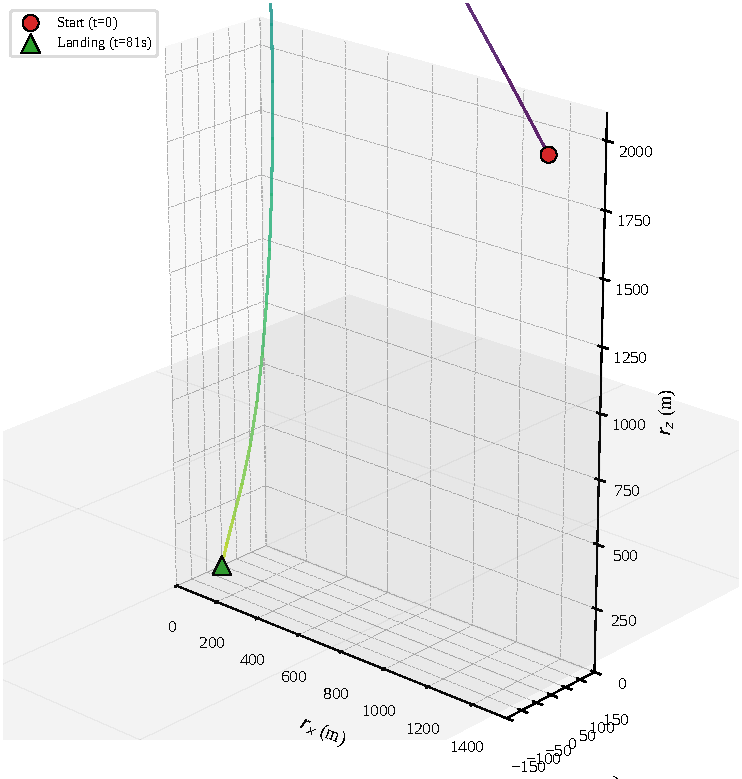
\includegraphics[width=\mediumfig]{figures/fig01_3d_trajectory.pdf}
\caption{三维着陆轨迹。起始于$(1500,0,2000)$ m，终止于原点。}
\label{fig:3d_trajectory}
\end{figure}

图 \ref{fig:3d_trajectory} 展示了着陆器在三维空间中的下降轨迹，起始于 $(1500, 0, 2000)$ m，三维路径平滑收敛至原点。轨迹在水平面（$yz$ 平面）的投影近乎是一条直线，表明最优解倾向于沿最短水平路径指向着陆点。图 \ref{fig:position_time} 给出了三轴位置随时间的变化曲线：$r_x$ 从 1500 m 单调递减至零，呈平滑抛物线外形——在前半段斜率较缓（接近零），在约 $t=30$ s 后斜率明显增大再逐渐归零；$r_y$ 始终维持在零附近，表明轨迹优化在水平 $y$ 方向几乎不产生机动，这与初始 $v_y = 0$ 且目标 $r_y=0$ 的对称边界条件一致；$r_z$ 从 2000 m 均匀下降至零，在终端附近斜率趋缓。该轨迹特征直观反映了下滑角锥约束对 $r_x$ 和 $r_z$ 之间比例关系的限制——$r_z$ 被约束在以 $r_x\tan\theta$ 为半径的锥体内，其中 $\theta = 86^{\circ}$，轨迹接近垂直下降。

\begin{figure}[tbp]
\centering
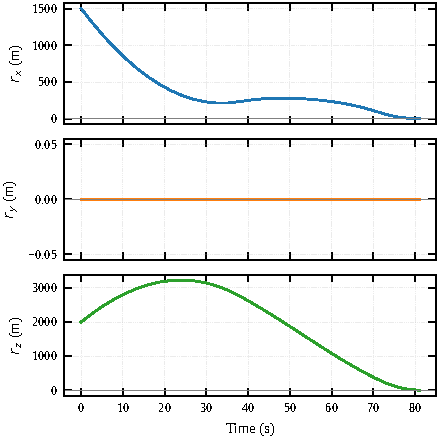
\includegraphics[width=\widefig]{figures/fig02_position_time.pdf}
\caption{非零位置分量时间曲线。上：$r_x$；下：$r_z$；对称边界使 $r_y$ 全程为零。}
\label{fig:position_time}
\end{figure}

图 \ref{fig:velocity_time} 显示速度分量的演化过程。$v_x$ 从初始的 -75 m/s 逐渐收敛至零，下降初期经历约 20 s 的加速段（负向速度绝对值从 75 增大至约 95 m/s），其后进入稳定减速段并在终端时刻归零。$v_x$ 先加速后减速的行为与最优燃料控制中典型的"先加速后减速"特征一致：在着陆前期，利用重力将势能转化为动能以提高发动机效率，在后期集中消耗燃料进行快速减速。$v_z$ 从 100 m/s 持续递减至零，减速过程贯穿整个 81 s 飞行时段，没有出现加速段——这是因为 $v_z$ 方向与重力方向垂直，不受重力助推作用。$v_y$ 始终为极小值（量级 $10^{-6}$ m/s）。速度剖面表明，着陆器的减速机动主要由推力在三轴上的分量配合实现，其中 $v_z$ 的衰减消耗了最大量的控制能量。

\begin{figure}[tbp]
\centering
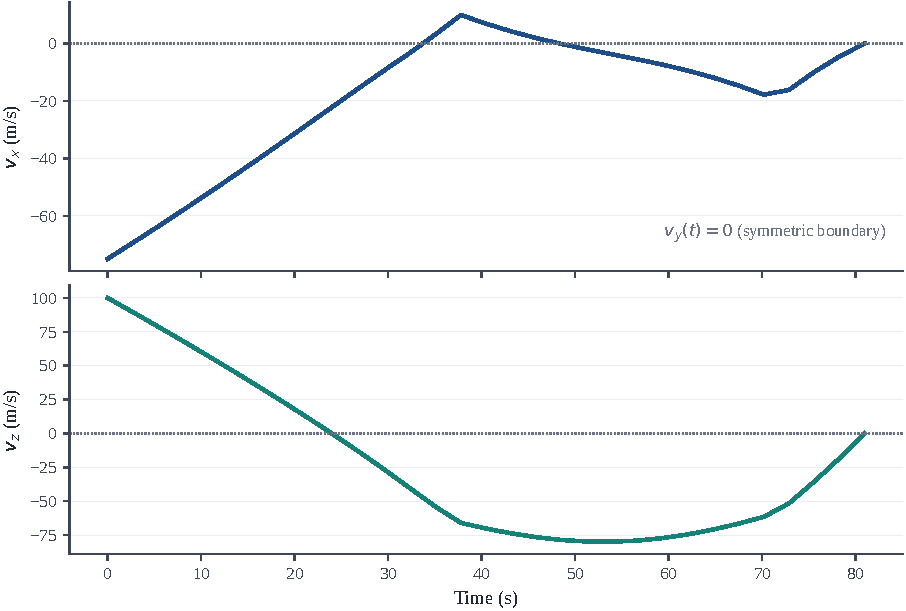
\includegraphics[width=\widefig]{figures/fig03_velocity_time.pdf}
\caption{非零速度分量时间曲线。上：$v_x$；下：$v_z$；对称边界使 $v_y$ 全程为零。}
\label{fig:velocity_time}
\end{figure}

图 \ref{fig:mass_evolution} 展示了当前标称数值解中着陆器质量从初始 1905.0 kg 至终端 1504.272 kg 的单调递减过程，对应目标值 400.728 kg（按一位小数记为 400.7 kg）。独立解审计同时发现，该终端质量低于 1505 kg 干重下界约 0.728 kg；因此 400.7 kg 只能作为各实现数值一致性的回归基准，不能表述为已满足全部物理约束的确认性燃料结果。质量曲线的斜率在大部分飞行时间内近乎恒定，仅在终端最后三步略有缓减，这描述了当前数值解的推力使用特征，但不消除上述干重违反。

\begin{figure}[tbp]
\centering
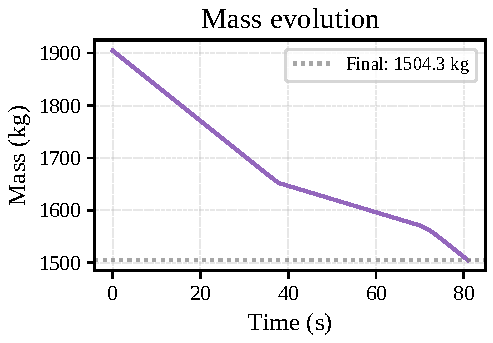
\includegraphics[width=\widefig]{figures/fig04_mass_evolution.pdf}
\caption{当前标称数值解的质量变化曲线。终端质量 1504.272 kg，低于 1505 kg 干重下界约 0.728 kg。}
\label{fig:mass_evolution}
\end{figure}

图 \ref{fig:thrust_comparison} 展示当前标称数值解中的推力幅值 $\|u\|$、松弛变量 $\sigma$ 与质量相关的推力上界。在绘图精度下，$\|u\|$ 与 $\sigma$ 在大部分控制区间接近，并在部分区间逼近上界。这可作为松弛间隙的数值诊断线索，但不能单独确认原非凸问题与 SOCP 的等价性~\cite{acikmese2013,acikmese2007lossless}。终端数步内推力幅值下降，记录峰值约为 8.66 N/kg。由于同一标称解存在干重下界违反，这些曲线只描述当前数值输出，不构成完整物理可行性结论。

\begin{figure}[tbp]
\centering
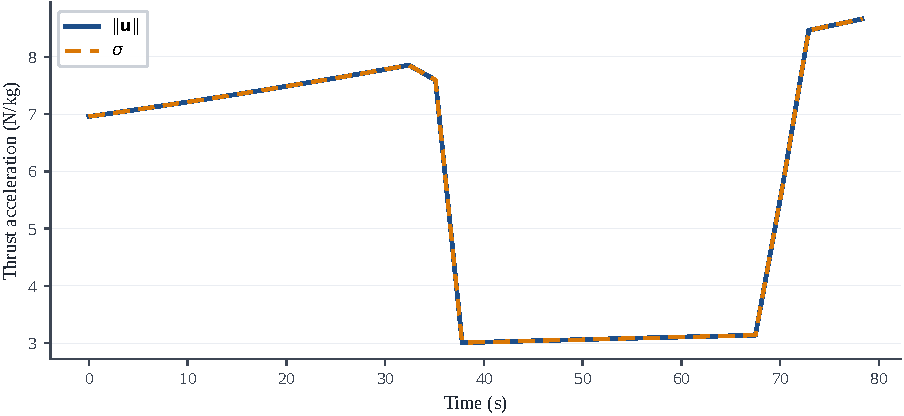
\includegraphics[width=\widefig]{figures/fig05_thrust_comparison.pdf}
\caption{当前标称数值解的推力幅值 $\|\bm{u}\|$ 与松弛变量 $\sigma$；二者的数值间隙用于诊断，不作为凸化无损性的独立证明。}
\label{fig:thrust_comparison}
\end{figure}

图 \ref{fig:glide_slope} 验证了下滑角约束的满足情况。上子图显示 $[r_y, r_z]$ 向量的范数与 $r_x\tan\theta$ 的关系，二者始终保持接触或分离；下子图给出了余量（$r_x\tan\theta - \|[r_y,r_z]\|$），该余量始终非负（$r_x\tan\theta \geq \|[y,z]\|$），在轨迹中段约束最为紧凑（余量在 $t=40$--60 s 区间接近零），说明下滑角约束在最优轨道的某些时刻确实起到了限制作用。特别值得注意的是，余量在全程均不严格为零但在轨迹中段逼近零，这表明下滑角约束对最优解施加了有效影响但并未全程激活——最优解在中段因物理条件自然趋近锥边界。

\begin{figure}[tbp]
\centering
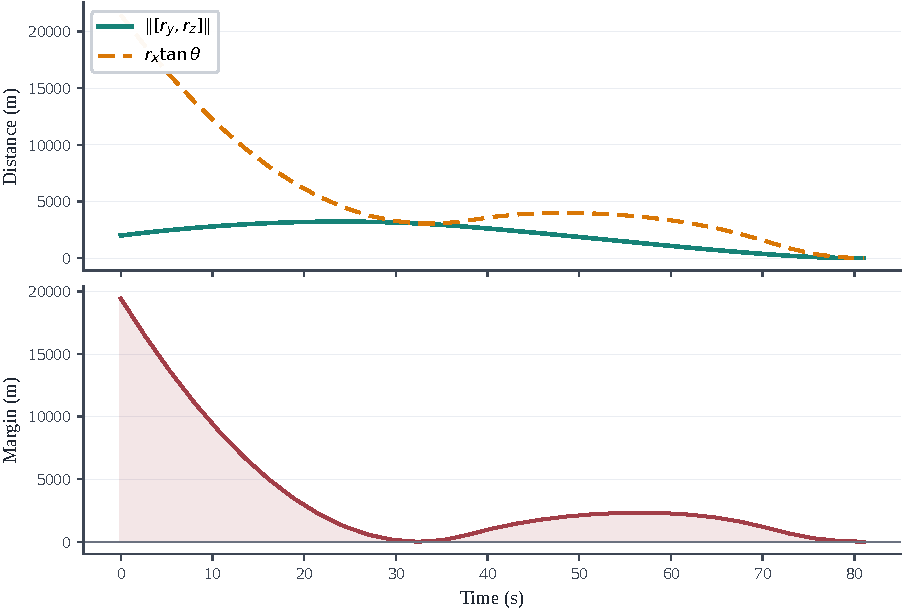
\includegraphics[width=\widefig]{figures/fig06_glide_slope.pdf}
\caption{下滑角约束验证。上：$\|[r_y,r_z]\|$ 与 $r_x\tan\theta$ 对比；下：约束余量。}
\label{fig:glide_slope}
\end{figure}

图 \ref{fig:thrust_cone} 验证了每个实际控制区间上的推力锥关系。上图中 $\sigma$ 与 $\|u\|$ 在视觉上重合；下图将其差值以科学计数法放大后显示，数值残差处于 $10^{-9}$ N/kg 量级，属于求解容差范围。终端节点不对应一个施加的控制区间，故未纳入该图的控制量比较。

\begin{figure}[tbp]
\centering
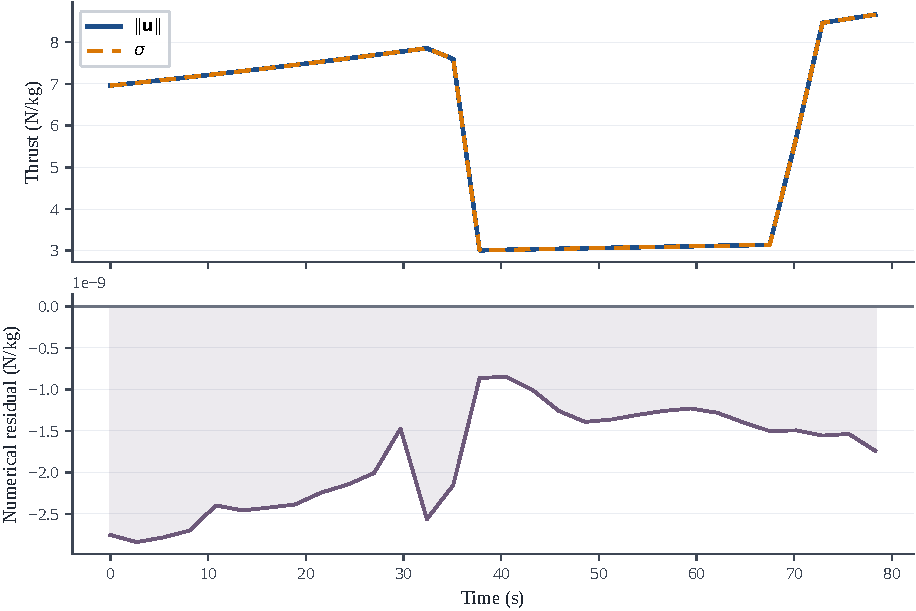
\includegraphics[width=\widefig]{figures/fig07_thrust_cone.pdf}
\caption{推力锥约束验证。上：实际控制区间上的 $\|\bm{u}\|$ 与 $\sigma$ 对比；下：数值残差 $\sigma - \|\bm{u}\|$。}
\label{fig:thrust_cone}
\end{figure}

\subsection{交叉验证}

\subsection{物理修正的自由终端时间与网格审计}

为避免把历史 $t_f=81$ s 手写基线的干重违反误读为物理可行结果，本文另建了物理修正的参数化研究模型（版本由 manifest 固定）。它在每个节点显式施加 $m\geq1505$ kg，并在每个控制区间的九个内部采样点施加下滑角 SOC 约束；固定 $(N,t_f)$ 的内层仍为 SOCP，终端时间由版本化 Decimal 网格外层搜索。该模型不修改、生成或替代 \texttt{MarsLanding/MarsLanding.c}；后者始终是 $N=30,t_f=81$ s 的原始、独立人工手写 CRS--CCS 参考实现。

图 \ref{fig:free_time_mesh} 从 75 条原始记录重算而来。N=20 的 15 个 ECOS 候选均明确不可行。N=30、40、60 分别得到最优已审计 ECOS 候选 $(t_f,\mathrm{fuel})=(78.02\,\mathrm{s},399.8010\,\mathrm{kg})$、$(78.02\,\mathrm{s},399.3954\,\mathrm{kg})$ 和 $(77.98\,\mathrm{s},398.9147\,\mathrm{kg})$。N=60 对应的 Clarabel 复算为 $398.9146$ kg，燃料差约 $2.1\times10^{-5}$ kg，且通过预注册审计。N=30、40 的 Clarabel 点分别因推力锥/包络残差略超过 $10^{-6}$ 门槛而被归为 \texttt{physical\_violation}；它们不能作为双求解器确认点。

\begin{figure}[tbp]
\centering
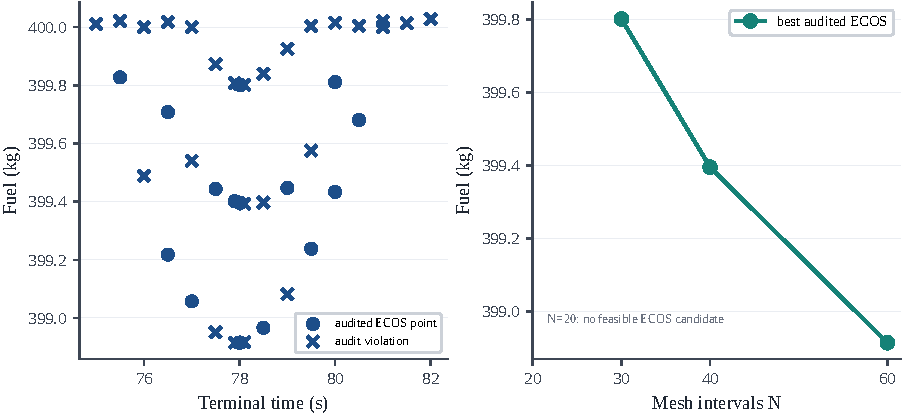
\includegraphics[width=\widefig]{figures/fig11_free_time_mesh.pdf}
\caption{物理修正自由终端时间研究。左：ECOS 候选的燃料--时间关系及分类；右：每个网格独立搜索得到的最佳已审计 ECOS 点。N=20 无可行点，且 N=30--60 的燃料仍随网格变化，故不能宣称连续时间最优或网格收敛。}
\label{fig:free_time_mesh}
\end{figure}

这项证据纠正了早期约 $399.733$ kg 的探索值：其节点约束虽可满足，但独立密集区间审计曾发现约 27.2 m 的下滑锥违反。加入区间 SOC 约束后，该数字不再可用。当前四网格数据也尚未满足连续三网格的预注册收敛阈值；它证明了模型缺陷被发现和修正，而不是已经完成连续时间最优性证明。

表 \ref{tab:cross_validation} 汇总仓库当前记录的六条数值路径，但其证据分为两个边界明确的集合。第一组是可由构建产物直接复核的三个 C ECOS 路径：手写矩阵 AVX 版、手写矩阵标量版和自动生成矩阵版。第二组是 \texttt{solver\_comparison.json} 中保存的三条 Python 路径：CVXPY+ECOS、CVXPY+Clarabel 和 CasADi+IPOPT。前两条 Python 路径求解 SOCP，IPOPT 使用 NLP 光滑等价形式。该表只陈述这些记录在燃料目标值上的数值一致性，不表示六条路径均由 quick CI 动态重跑，也不表示它们已通过全部物理残差审计。

\begin{table}[tbp]
\centering
\caption{六条求解路径的记录值及其数值对比}
\label{tab:cross_validation}
\begin{tabular}{lclrr}
\toprule
求解方案 & 问题类型 & 建模方式 & 燃料消耗 (kg) & 偏差 (\%) \\
\midrule
ECOS AVX（C 手写） & SOCP & 手写稀疏 CCS 矩阵 & 400.7 & 基准 \\
ECOS 标量（C 手写） & SOCP & 手写稀疏 CCS 矩阵 & 400.7 & 0.0 \\
ECOS（C 自动生成） & SOCP & CasADi 生成 CCS 矩阵 & 400.7 & 0.0 \\
CVXPY+ECOS & SOCP & CVXPY 高阶建模 & 400.7 & 0.0 \\
CVXPY+Clarabel & SOCP & CVXPY 高阶建模 & 400.7 & 0.0 \\
CasADi+IPOPT & NLP & 光滑等价 SOC $\to$ NLP & 400.7 & 0.0 \\
\bottomrule
\end{tabular}
\end{table}

三个 C 可执行路径当前均报告 400.7 kg；Python comparison 文件中的三条记录也均为 400.7 kg。这里的 0.0\% 是按一位小数记录后的目标值差异，不应解读为高精度逐位相等。尤其是，这一一致性不消除前述标称解约 0.728 kg 的干重下界违反。

\begin{figure}[tbp]
\centering
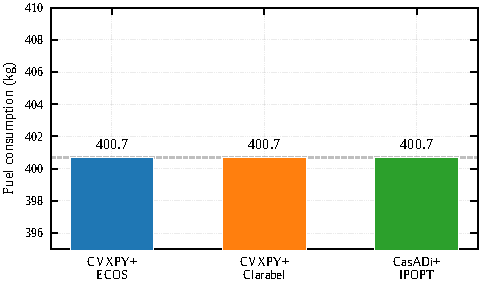
\includegraphics[width=\widefig]{figures/fig08_fuel_comparison.pdf}
\caption{Python comparison 文件中的三条燃料目标值记录；按一位小数均为 400.7 kg。}
\label{fig:fuel_comparison}
\end{figure}

这两个证据集合为实现一致性提供了交叉检查，但不足以单独证明算法或物理模型正确。C 手写版与自动生成版保持独立：前者以 CRS\_PUSH 宏逐行组装并转换为 CCS，后者使用 CasADi 生成的 CCS 数据；CVXPY 则通过约束表达式规范化生成问题。它们得到相同的一位小数目标值，可以发现明显的装配或符号回归，但不能排除小于显示精度的差异，也不能替代约束残差审计。

Python comparison 中 ECOS 与 Clarabel 的记录值一致，说明该数据快照没有显示求解器级别的一位小数偏差。由于 quick CI 不动态运行 Clarabel 或 IPOPT，这一结论严格限于版本库中的 comparison 文件；环境、依赖或模型变化后必须重新生成证据，不能由静态快照外推。

CasADi+IPOPT 的记录值与 SOCP 路径相同，可作为光滑 NLP 路径的历史数值对照；但静态记录本身不能构成无损凸化等价性的最终确认。该判断还需要可重放的求解输出、锥松弛间隙和全部物理约束残差共同支持~\cite{acikmese2013}。

需要特别指出的是，IPOPT 版本使用光滑等价形式（$t^2 - x^\top x \geq 0$）替代二阶锥约束。该转换要求在 $t \geq 0$ 条件下确保 $t^2 - x^\top x \geq 0$ 与原锥约束 $\|x\|\leq t$ 完全等价。曾在实验早期尝试将 SOC 约束错误地拆分为标量不等式 $r_x \geq 0$、$r_y \geq 0$、$r_z \geq 0$，结果导致燃料消耗偏差高达 23\%，因为该拆分完全丢失了范数约束的耦合关系，仅限制了位置符号而未约束其范数。这一教训再次强调了锥约束作为整体处理的必要性。

\subsection{计算性能分析}

求解时间是评估部署可行性的一个指标，但必须限定计时范围和运行环境。火星着陆动力下降段持续时间约 60--90 s，制导重规划常以 1--10 Hz 为设计参考。表 \ref{tab:performance} 汇总五条现有计时记录；C 路径统计预初始化后 1000 次重复 \texttt{ECOS\_solve} 的平均 CPU 时间，Python 条目则包含各自记录路径的上层调用开销，因此两组数值不属于严格同口径端到端基准。

\begin{table}[tbp]
\centering
\caption{计算性能对比（1000 次重复测量均值）}
\label{tab:performance}
\begin{tabular}{lrc}
\toprule
求解方案 & 单次求解耗时 (ms) & 相对基准 \\
\midrule
ECOS AVX（C 手写，冻结均值） & 7.361 & 限定均值 \\
CVXPY+ECOS & 372.22 & $\times$46.5 \\
CVXPY+Clarabel & 348.06 & $\times$43.5 \\
CasADi+IPOPT & 5835.4 & $\times$729 \\
\bottomrule
\end{tabular}
\end{table}

冻结报告中的 C 手写 AVX 目标均值为 7.361 ms/次。该值由 \texttt{clock()} 累计 setup 后 1000 次 \texttt{ECOS\_solve} 的 CPU 时间得到；没有逐次 raw samples，不能据此报告 p99、最大值或 WCET，也不是端到端重规划延迟。

\begin{figure}[tbp]
\centering
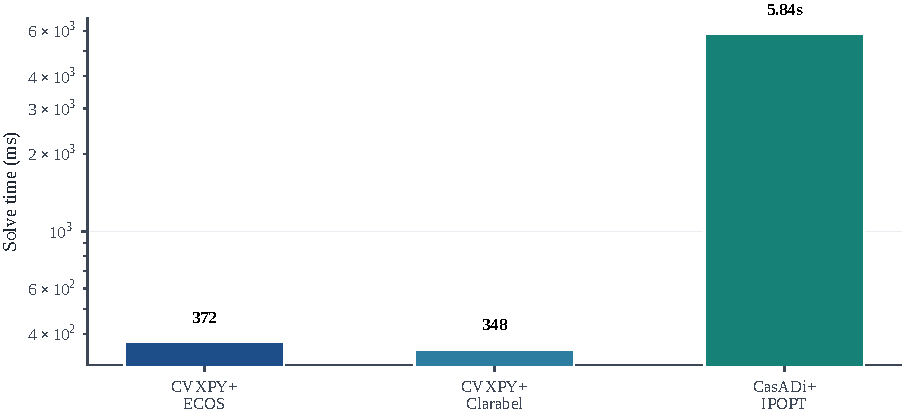
\includegraphics[width=\widefig]{figures/fig09_time_comparison.pdf}
\caption{三种 Python 求解路径的单次求解耗时对比（对数坐标）。}
\label{fig:time_comparison}
\end{figure}先前标量与 AVX/FMA 构建约 2.4\% 的差异没有冻结 raw timing 或硬件计数器支持，现仅保留为待复现实验，不作 SIMD 因果结论。

CVXPY 建模层的引入使测得时间从约 8 ms 增至约 350--370 ms（约 45 倍）。这一差距表明，对小规模 SOCP，建模、规范化和结果回提取会显著影响端到端 Python 调用时间。CVXPY 的调用路径包括约束表达式构造、DCP 分析、规范化、稀疏矩阵组装、求解器调用和结果回提取；该开销适合离线设计，但不宜直接用于星上实时制导。CasADi+IPOPT 耗时约 5.8 s，是三类方案中最慢者，主要因为 NLP 迭代需要反复评估 Jacobian 和 Hessian 矩阵，更适合地面离线校核。

在 SOCP 求解器层面，Clarabel（348 ms）相比 ECOS（372 ms）在 CVXPY 环境下快约 6.5\%。Clarabel 作为 Rust 实现的新型内点法求解器，其 LDL 分解采用了更加缓存友好的超节点（supernodal）策略，减少了内存引用局部性差的间接索引次数。然而，当脱离 CVXPY 建模层并在预初始化工作区上重复调用时，ECOS 的 C 原生接口仍表现出明显优势（约 8 ms）。手写问题数据采用栈上定长数组；ECOS 工作区本身仍由 \texttt{ECOS\_setup()} 分配，硬实时部署需进一步采用静态内存池改造。

\subsection{单精度与双精度对比}

不同嵌入式处理器对单精度和双精度的硬件支持差异较大，具体代价必须以芯片手册和目标构建测量为准。本文仅比较仓库中两组 Clarabel 配置的记录结果，不将其直接外推到硬件选型。

现有记录中，\texttt{Clarabel f32} 使用放宽至 $10^{-6}$ 的容差，\texttt{Clarabel f64} 使用默认配置。由于精度和容差同时变化，这不是控制变量实验。

\begin{figure}[tbp]
\centering
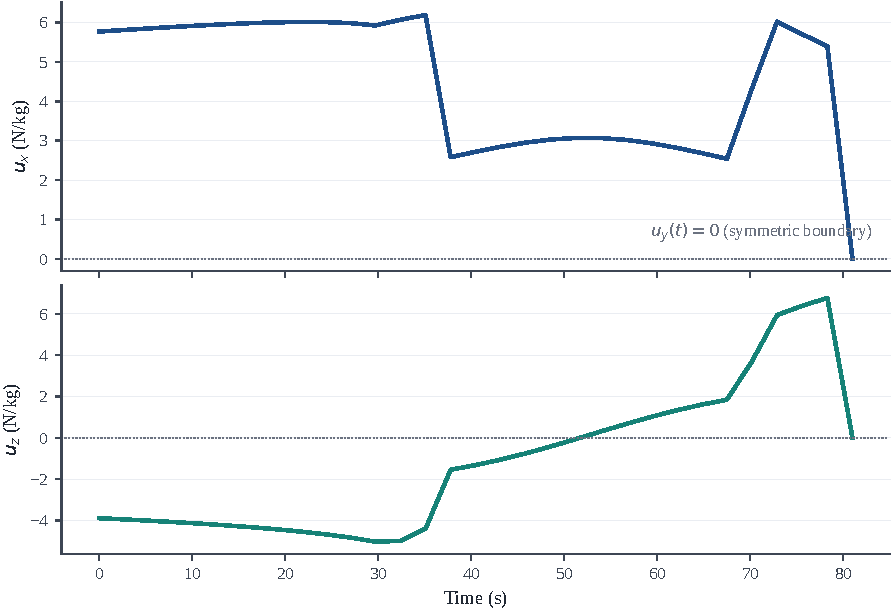
\includegraphics[width=\widefig]{figures/fig10_control_time.pdf}
\caption{非零控制加速度分量 $u_x$、$u_z$ 的时间演化曲线；对称边界使 $u_y$ 全程为零。}
\label{fig:control_time}
\end{figure}

两组不同配置分别记录 1880+ kg 和 400.7 kg，名义差异约 375\%。该观测不能单独归因于浮点精度，也不能在缺少同容差残差审计时断言 KKT 系统崩溃。分离精度影响需要统一模型、容差、缩放、停止条件和审计指标。

变量量级从位置约 $10^3$ m 到 $\exp(-z)$ 约 $5\times10^{-4}$，提示缩放和条件数可能影响数值行为，但这只是诊断假设。另一个可直接计算的局部关系是 $m=\exp(z)$ 下 $dm/dz=m$：在本问题质量约 1500 kg 时，给定的 $z$ 误差会在一阶换算中乘以约 1500。该关系只是局部误差单位换算，不说明自动微分、梯度或 Hessian 被放大同样倍数，也不能解释两组 Clarabel 配置的全部差异。后续应在统一容差下分别测试缩放、精度和残差。

\subsection{蒙特卡洛鲁棒性分析}

先前无冻结数据支持的 Monte Carlo 数字已撤回。现已按 canonical manifest 完成并冻结 1000 个逐样本记录；求解器状态与物理审计分类保持分离。

后续确认实验采用仓库中的 canonical manifest \texttt{near\_nominal\_v1.json}：随机种子固定为 42，计划样本数为 1000；标称初始条件为 $r_0=(1500,0,2000)$ m、$v_0=(-75,0,100)$ m/s；仅对 $r_x,r_z$ 施加半宽 200 m 的均匀增量扰动，仅对 $v_x,v_z$ 施加半宽 20 m/s 的均匀增量扰动，两个 $y$ 分量保持不变。每个样本均由 CVXPY+ECOS 求解，并保存输入、求解器状态、耗时、manifest 摘要和审计指标。

1000 个尝试中，483 个为 \texttt{success}，363 个为 \texttt{physical\_\allowbreak violation}，153 个为 \texttt{solver\_\allowbreak infeasible}，1 个为 \texttt{solver\_error}。审计成功率为 0.483，Wilson 95\% 区间为 $[0.4522,0.5140]$。仅对 483 个成功样本计算的燃料条件分布为：均值 383.8378 kg、样本标准差 9.5240 kg、最小值 360.2158 kg、最大值 399.9547 kg。该条件统计不包含失败样本，不能表述为总体燃料分布或鲁棒性通过。单个 \texttt{solver\_error} 尚未归因，需结合原始记录后续调查。

\section{嵌入式部署讨论}

\subsection{嵌入式硬件平台分析}

本章讨论将前文实现的稀疏 ECOS 求解算法部署至嵌入式飞行计算机的可行性。当前算法开发与验证依托于 Intel N150 平台（Gracemont 小核架构，8 GB RAM），该平台功耗约 6\textasciitilde{}10 W，属于 x86 低功耗产品线。然而，实际航天飞行计算机通常采用 ARM Cortex-M 或 RISC-V 内核的微控制器（MCU），其计算资源较 N150 低数个数量级，对算法及实现有完全不同的约束。

目标部署平台选用 ARM Cortex-M7 内核微控制器。Cortex-M7 是 ARMv7-M 架构中性能最高的 MCU 内核，支持双精度浮点运算单元（FPU），主频通常为 200\textasciitilde{}600 MHz，典型片上 SRAM 为 512 KB\textasciitilde{}2 MB。对于火星着陆这类航天制导控制应用，选用具备双精度 FPU 的 M7 而非 M4（单精度 FPU）或 M3（无硬件 FPU）至关重要。

双精度浮点运算的强制性已在实践中得到充分验证。本课题组此前在 Clarabel 求解器上进行了单精度（float）对比实验：相同 SOCP 问题、相同锥约束，仅将求解器数值类型从 double 切换为 float，所得燃料消耗从 400.7 kg 剧增至 1880+ kg，相对误差达 375\%。这一巨大偏差的根本原因在于该问题的数值动态范围极端：位置状态量级约 $10^3$ m，而质量对数状态 $\ln m$ 的下界约 $7.3$，其指数 $\exp(-z)$ 量级仅约 $10^{-4}$，贯穿 KKT 系统的条件数达到 $10^8$。IEEE 754 单精度浮点数仅约 7 位有效十进制数字，在 $10^8$ 条件数下求解线性系统时损失的精度远超收敛容差。双精度提供约 16 位有效数字，可安全容纳此动态范围。因此目标平台必须配备双精度 FPU，Cortex-M7 的 FPv5 硬浮点单元满足此需求。

M7 内核的双精度 FPU 采用单发射流水线，双精度乘法延迟通常为 3\textasciitilde{}5 周期，双精度除法为 15\textasciitilde{}20 周期，显著慢于单精度但远优于软件浮点模拟（后者每次运算需数百周期）。ECOS 求解器的核心计算负载为 LDL 稀疏分解和三角回代，其运算模式为稀疏点积与标量除法，硬浮点支持可将这些操作缩短至数十纳秒量级。

\subsection{内存占用分析}

嵌入式 MCU 的内存约束是算法部署面临的核心挑战。片上 SRAM 以 MB 计，不同于 N150 平台数 GB 的 DDR 内存，必须逐字节精打细算。

KKT 系统是内存占用的主要来源。该问题的 KKT 矩阵维度为 $1023 \times 1023$（对应 341 个变量的原始-对偶系统），对 ECOS 使用 LDL 分解的 KKT 格式而言，仅存储上三角部分。当前手写版构造的 KKT 上三角非零元约 2531 个，各非零元以双精度浮点数（8 字节）配合行列索引（int，各 4 字节）存储，采用压缩列存储（CCS）格式。CCS 格式由列指针（$n+1=1024$ 个 int）、行索引（nnz 个 int）、数值（nnz 个 double）三数组组成，对 2531 非零元的存储开销约为：

\begin{align}
\text{CCS\_KKT} &= 1024 \times 4 + 2531 \times (4 + 8) = 34.4\ \text{KB}.
\end{align}

LDL 因子 $\bm{L}$ 的填充（fill-in）是主要不确定因素。通过近似最小度（AMD）排序可以显著减少填充量。ECOS 内部集成了 AMD 预处理，在典型火星着陆问题中，$\bm{L}$ 的非零元填充至约 5000\textasciitilde{}15000，稀疏度取决于 AMD 排序的有效性和 KKT 矩阵的结构。LDL 因子同样以 CCS 格式存储，按上限 15000 非零元估算：

\begin{align}
\text{CCS\_L} &= (n+1) \times 4 + 15000 \times (4 + 8) \approx 184.0\ \text{KB}.
\end{align}

求解器运行时还需要若干工作向量：残差向量（$n$ 个 double，约 8 KB）、搜索方向（$n+1$ 个 double，约 8 KB）、原始与对偶变量（各 $n$ 个 double，约 16 KB）、锥投影临时变量等，合计约 50\textasciitilde{}70 KB。叠加 KKT 与 LDL 因子后，ECOS 求解器总堆内存需求为：

\begin{align}
M_{\text{total}} &= M_{\text{KKT}} + M_{\text{L}} + M_{\text{workspace}} \approx 34 + 184 + 70 = 288\ \text{KB}.
\end{align}

考虑实际运行时的临时缓冲区和内存碎片，安全估计为 400\textasciitilde{}700 KB。对于典型配置 1 MB SRAM 的 Cortex-M7（如 STM32H7 系列），这一需求占总量约 40\textasciitilde{}70\%，可以容纳，但已无充裕余量。

当前 ECOS 求解器使用标准库的 \texttt{malloc}/\texttt{free} 进行动态内存分配。在空间应用中，动态内存分配存在两大风险：一是内存碎片化导致长时间运行后分配失败；二是分配时间不可预测，违背硬实时约束。为此，必须将动态分配改造为编译期预分配的静态内存池。

改造方案如下：基于目标问题的维度（变量数 $n=341$、约束数 $m=341$、非零元数等），通过离线的内存预算分析，预计算 LDL 分解在最坏情况下的填充上限。在初始化阶段从静态池中一次性分配所有缓冲区，求解过程中不再进行任何动态分配。静态池的大小在编译期确定，作为宏定义写入头文件：

\begin{align}
\#\text{define STATIC\_POOL\_SIZE}\ (1024 * 700) \quad //\ 700\ \text{KB}
\end{align}

将 ECOS 的 \texttt{stgl\_alloc()} 和 \texttt{stgl\_free()} 替换为静态池的指针偏移分配器，即可完全消除运行时动态分配。

\subsection{实时性分析}

火星动力下降的制导周期通常为 100\textasciitilde{}500 ms，远快于飞行器的刚体动力学时间常数（秒级）。这一周期为 SOCP 求解提供了充足的计算时间窗口。

Intel N150 平台实测单次 ECOS 求解平均耗时约 8 $\mu$s（取内点法迭代次数 8\textasciitilde{}12 次均值，Release 模式）。移植至 Cortex-M7 后的性能可通过运算特征估算。分析 ECOS 求解器的计算热点分布如表 \ref{tab:ecos_hotspots} 所示。

\begin{table}[htbp]
\centering
\caption{ECOS 求解器计算热点分布}
\label{tab:ecos_hotspots}
\begin{tabular}{clc}
\toprule
计算阶段 & 操作特征 & N150 耗时占比 \\
\midrule
LDL 分解 & 稀疏点积、除法（内存延迟主导） & 45\textasciitilde{}55\% \\
三角回代 & 稀疏前代/回代（内存延迟主导） & 15\textasciitilde{}20\% \\
KKT 组装 & 矩阵向量运算 & 10\textasciitilde{}15\% \\
锥投影 & 标量运算、分支判断 & 5\textasciitilde{}10\% \\
余项计算 & 向量点积、2-范数 & 5\textasciitilde{}10\% \\
\bottomrule
\end{tabular}
\end{table}

稀疏 LDL 分解和三角回代是耗时最长的两个阶段，均以稀疏矩阵向量运算为主。在 N150 上，这些操作的核心瓶颈是内存带宽而非计算吞吐——不规则的内存访问模式（CCS 格式的 gather/scatter）使得处理器频繁等待缓存未命中。Cortex-M7 的 SRAM 通常挂载在紧耦合内存总线上，访问延迟低（通常在 2\textasciitilde{}5 周期），无 DDR 的片外访问延迟。因此，在同样 8 次迭代、同样问题规模下，M7 上的内存延迟惩罚较小，但主频差距显著。

估算目标性能时遵循以下假设：N150（Gracemont 小核）等效单线程性能约 4000 DMIPS，Cortex-M7 在 480 MHz 下约 1200 DMIPS，两者比值为 3.3。LDL 分解的 O(nnz) 模型中计算与访存交织，实际 IPC 差异相对较小，保守估计综合性能比为 5\textasciitilde{}10 倍。由此得：

\begin{align}
t_{\text{M7}} = 8\ \mu\text{s} \times (5 \sim 10) \approx 40 \sim 80\ \mu\text{s}.
\end{align}

但上述估算未考虑 LLVM/GCC 向量化和架构差异，更保守的上限估计考虑 Cortex-M7 无 SIMD 单元且分支预测能力较弱，给出 200\textasciitilde{}500 $\mu$s 的单次求解时间。

即使取最保守估计 500 $\mu$s，与 100 ms 的制导周期相比仅占 0.5\%。在周期剩余部分，飞行计算机还需完成导航滤波（通常为扩展卡尔曼滤波器，约需 1\textasciitilde{}5 ms）、姿态控制律计算（约需 0.1\textasciitilde{}0.5 ms）、遥测数据打包等任务。图 \ref{fig:timing_budget} 展示了完整周期的时间预算分配。

\begin{figure}[htbp]
\centering
\begin{tikzpicture}[scale=0.6]
  \draw[thick] (0,0) -- (20,0);
  \foreach \x in {0,2,...,20} \draw (\x,-0.1) -- (\x,0.1);
  \node[above] at (0,0.3) {0 ms};
  \node[above] at (10,0.3) {50 ms};
  \node[above] at (20,0.3) {100 ms};

  \fill[blue!30] (0,0.5) rectangle (0.01,1.0);
  \node[above] at (0.005,1.1) {\tiny SOCP};

  \fill[green!30] (0.5,0.5) rectangle (5.5,1.0);
  \node[above] at (3.0,1.1) {\tiny 导航滤波};

  \fill[orange!30] (6.0,0.5) rectangle (6.5,1.0);
  \node[above] at (6.25,1.1) {\tiny 姿态控制};

  \fill[gray!20] (7.0,0.5) rectangle (8.5,1.0);
  \node[above] at (7.75,1.1) {\tiny 余量};
\end{tikzpicture}
\caption{制导周期时间预算分配（100 ms 周期）}
\label{fig:timing_budget}
\end{figure}

此外，SOCP 求解之前的矩阵构造阶段（将问题状态量组装为 KKT 系统）可忽略不计。当前手写 C 版本的矩阵构造采用预计算的符号非零元结构，每次求解仅需回调约 3400 次浮点赋值操作，实测耗时小于 0.01 ms。该阶段无需 CSP（约束满足问题）求解或动态数据结构的构建，在 M7 上预计也仅需 0.05\textasciitilde{}0.1 ms。

值得注意的是，ECOS 内点法的迭代次数受问题数值条件影响：在终端接近精确着陆条件时，KKT 矩阵可能发生近奇异现象，导致迭代次数增加至 15\textasciitilde{}20 次。极端情况下，纯内点法可能需要额外的迭代精化（iterative refinement）步骤以恢复数值精度。ECOS 默认的迭代精化步数为 9（参见参数 \texttt{NITREF}），若保留此设置，每次迭代精化相当于一次额外的三角回代，对总求解时间影响约 15\textasciitilde{}25\%。

\subsection{交叉编译策略}

将 ECOS 求解器部署至 Cortex-M7 需要完整的交叉编译工具链支持。项目选用 \texttt{arm-none-eabi-gcc} 工具链配合 Newlib C 标准库实现。

工具链配置的核心是目标 Triple 的选择。Cortex-M7 支持双精度 FPU，使用 ARMv7-M 架构的 FPv5 扩展，对应的 GCC 选项为：

\begin{align}
\text{CFLAGS} &= \texttt{-mcpu=cortex-m7 -mthumb} \notag \\
&\quad \texttt{-mfloat-abi=hard -mfpu=fpv5-d16} \notag \\
&\quad \texttt{-Os -ffunction-sections -fdata-sections}.
\end{align}

其中 \texttt{-mfloat-abi=hard} 使用硬浮点调用约定，所有浮点参数通过 FPU 寄存器传递，避免通过通用寄存器转发的开销。\texttt{-mfpu=fpv5-d16} 表示使用包含 16 个双精度寄存器的 FPv5 扩展。\texttt{-Os} 优化尺寸模式对嵌入式部署至关重要：MCU 的 Flash 容量通常为 1\textasciitilde{}2 MB，而 ECOS 核心代码约 8000 行，经 \texttt{-Os} 编译后二进制体积可压缩至约 100\textasciitilde{}150 KB。

\texttt{arm-none-eabi-newlib} 作为 C 标准库运行时，提供基本的数学函数实现。ECOS 求解器依赖 \texttt{<math.h>} 中的 \texttt{sqrt}、\texttt{exp}、\texttt{pow} 等函数。Newlib 的数学库分为双精度（libm.a）和单精度（libm\_f.a）两套实现，链接时需确保使用双精度版本：

\begin{align}
\texttt{LIBS} &= \texttt{-lm -lc -lgcc}.
\end{align}

Newlib 的 \texttt{sqrt} 和 \texttt{exp} 在 ARM 架构下通常调用硬浮点指令（VSQRT.F64 和 VEXP.F64 或软件模拟），其性能取决于 M7 内核是否实现这些指令。Cortex-M7 的 FPv5 支持 VSQRT 指令，双精度平方根延迟约 20 周期；指数函数通常通过查表加多项式逼近实现，约需 50\textasciitilde{}100 周期。

如前文所述，必须替换 \texttt{malloc}/\texttt{free}。ECOS 的内存分配集中于少数几个固定大小的缓冲区，适合采用极简的静态池方案。改造在 ECOS 的 \texttt{include/ecos/glblopts.h} 中添加预分配宏：

\begin{align}
\#\text{define USE\_STATIC\_POOL}\ 1
\end{align}

并在 \texttt{src/cone.c} 中将 \texttt{stgl\_alloc} 替换为：

\begin{align}
\#\text{define stgl\_alloc(s)}\ \_\_pool\_alloc(s)
\#\text{define stgl\_free(p)}\ \_\_pool\_free(p)
\end{align}

其中 \texttt{\_\_pool\_alloc} 及 \texttt{\_\_pool\_free} 的实现仅在静态缓冲区内做指针偏移与回滚，单次分配/释放仅需约 5\textasciitilde{}10 条指令，无锁、无碎片、O(1) 时间复杂度。

\subsection{飞行计算机集成路线}

将上述 SOCP 求解算法集成至完整的飞行计算机软件栈中，涉及导航、制导、控制三层的闭环工作流程。对于火星动力下降阶段，典型的计算流程如下：

\begin{enumerate}
  \item \textbf{导航滤波器}：接收 IMU 加速度计与陀螺仪数据，结合雷达高度计或视觉测距（如 NASA 的 Lander Vision System）给出飞行器位置 $\bm{r}$、速度 $\bm{v}$、姿态的估计值，更新频率通常为 100\textasciitilde{}1000 Hz。
  \item \textbf{SOCP 轨迹生成}：以导航滤波器输出的当前状态作为初始条件，调用 ECOS 求解器重新求解 SOCP 问题，生成当前到终端状态的最优轨迹。此步骤执行频率较低（10 Hz，即每 100 ms 一次），与制导周期匹配。
  \item \textbf{姿态控制器}：从 SOCP 输出的推力向量 $\bm{u}^*$ 解析出期望推力大小和方向，通过姿态控制律（通常为 PD/PID 或滑模控制）分配到 6 台发动机的点火指令。
  \item \textbf{故障检测与重规划}：实时监测导航状态与 SOCP 预测轨迹的偏差。当偏差超过预设阈值（如位置偏差 $> 50$ m 或速度偏差 $> 10$ m/s），触发重规划信号，强制进入下一制导周期重新求解 SOCP。
\end{enumerate}

在以上流程中，SOCP 求解结果的质量直接决定着陆精度。当前 3-DOF 模型求解输出的期望推力 $\bm{u}^*$ 需要转换为姿态指令（期望俯仰角和偏航角），由姿态内环跟踪。由于姿态响应时间远快于位置动力学（通常姿态时间常数 $< 0.5$ s，而位置时间常数约 5\textasciitilde{}10 s），姿态跟踪延迟对制导精度的影响可忽略。

故障检测与重规划机制是安全关键系统的核心保障。当大气密度、风速等环境参数偏离标称值，或发动机实际推力与标称值出现偏差时，制导律必须能够在线调整。当前 SOCP 问题每次求解所需的 200\textasciitilde{}500 $\mu$s 使得重规划可在同一控制周期内完成，无需跨周期等待。这一能力相比传统基于查表或离线轨迹跟踪的制导方案提供了显著更强的鲁棒性。

\subsection{当前局限与未来工作}

当前实现存在若干简化假设，以下分别讨论其对实际飞行的影响及后续改进方向。

\textbf{无大气阻力模型}：当前动力学模型完全忽略大气阻力。火星大气密度极低，仅为地球的约 1\%（表面大气压约 600 Pa），在动力下降段飞行速度从约 150 m/s 降至 0，动压峰值约 100\textasciitilde{}300 Pa，对应阻力加速度约 $0.01\sim0.1\,\text{m/s}^2$，与火星重力（$3.7114\ \text{m/s}^2$）相比小 1\textasciitilde{}2 个数量级。在燃料优化问题中忽略此量级的阻力导致的终端位置偏差约 1\textasciitilde{}5 m，在可接受范围内。

\textbf{3-DOF 质点模型，无姿态耦合}：当前模型将飞行器简化为质点，仅考虑平动动力学，忽略姿态与推力的耦合效应。实际飞行中，推力方向受限于飞行器当前的姿态角速率和最大角加速度，不能瞬时改变。单台发动机的推力方向固定（安装倾角 ${27}^{\circ}$），合力方向由各台发动机的节流分配共同决定，存在耦合约束。将 3-DOF 模型扩展为 6-DOF 刚体模型（包含 3 个平动自由度和 3 个转动自由度）将使问题维度大幅增加——每步决策变量从 11 维增至 18 维，约束数量相应增加。SOCP 问题规模预计膨胀至约 $n=558$、$m=558$，KkT 矩阵非零元约 4000\textasciitilde{}6000。但 ECOS 求解器的稀疏 LDL 分解算法及 AMD 排序能力仍可应对这一规模，单次求解时间预计在 Cortex-M7 上仍低于 5 ms，不影响 100 ms 的制导周期。

\textbf{固定终端时间，未优化着陆时间}：当前终端时间 $t_f = 81$ s 为固定值，由离线预设确定。实际任务中，最优着陆时间随初始状态和气象条件而变化。若将 $t_f$ 纳入优化变量，问题将从定终端时间的最优控制变为变终端时间问题。一种处理策略是将 $t_f$ 作为外层搜索变量，由黄金分割法或二分法在合理区间（如 70\textasciitilde{}100 s）内迭代调用 ECOS 求解。外层搜索通常仅需 5\textasciitilde{}10 次迭代，每次迭代需求解一次 SOCP，总计算时间约 5\textasciitilde{}10 ms，仍在可接受范围内。

上述局限为后续工作指明了三个方向：引入大气阻力模型（通过增加海拔高度相关的指数密度剖面）、将 SOCP 拓展至 6-DOF 刚体模型（需处理姿态与推力之间的旋转耦合约束）、以及变终端时间外层优化。这三项增强可逐步集成，每项增强对求解时间的影响均可通过前文所述的方法进行预算与验证。

\section{结论}

本文建立并审计了一个火星动力下降 SOCP 研究 artifact。其不可替代的工程资产是原始手写 C 源：作者独立、人工维护的 CRS 稀疏矩阵构造及 CRS--CCS 转换实现（\texttt{MarsLanding.c}）。自动生成 C 数据与 Python 路径仅用于一致性交叉验证，不能替代该资产。

历史固定时间手写基线在多条数值路径中给出 400.7 kg 的一位小数目标一致性，但独立审计发现其终端质量低于干重下界约 0.728 kg。因此该数值被保留为 numerical golden，而不作为物理可行燃料结论。

为处理这一问题，本文新增显式干重和区间内下滑锥约束的参数化固定时间 SOCP，并以冻结的自由终端时间网格研究审计 75 条尝试。N=20 无可行 ECOS 候选；N=30、40、60 的最佳已审计 ECOS 点仍随网格变化。只有 N=60 的 ECOS/Clarabel 复算同时通过预注册审计，约为 398.915 kg。该结果表明区间约束和独立审计能够发现节点模型遗漏，但尚不能证明连续时间最优或网格收敛。

工程上，N150 主机的 7.361 ms 仅覆盖 setup 后的 \texttt{ECOS\_solve()} 平均 CPU 时间。本文不支持 p99 或 WCET，也没有目标硬件、内存或端到端证据，因而不主张飞控部署已经完成。下一阶段应先完成同配置 f32/f64 控制实验、目标平台分阶段计时和内存测量，再进行版本化闭环 Monte Carlo、故障注入与安全降级验证。


% --- 参考文献 ---
\bibliographystyle{ieeetr}
\bibliography{refs,refs_mission}

\end{document}
